\documentclass{beamer}
\usepackage{graphicx}
\usepackage{amsmath}
\usepackage{booktabs}
\usepackage{amsmath,amssymb,amstext,amsthm,amsmath,amssymb,amsfonts} % Lots of math symbols and environments
% \usepackage[pdftex,pagebackref=false]{hyperref} % with
\usepackage{colortbl}
% \usepackage{algorithm2e}
% \usepackage[ruled,vlined,linesnumbered]{algorithm2e}
\usepackage{array}
\usepackage{booktabs}
\usepackage{geometry}
% \geometry{margin=0.5in}
\usepackage{adjustbox}
\usepackage{longtable}
\usepackage{tikz}
\usepackage{subcaption}
\usepackage{hyperref}
\usepackage{algorithm}
% \usepackage{algorithmic}
\usepackage{algpseudocode}
% \usepackage{comment}
\usepackage{caption}
\usepackage{float}

\usetheme{AnnArbor}
% \usecolortheme{default}

\title[Challenges in RL]{MAC Thesis -- From Theory to Practice: Challenges in Reinforcement Learning\\[1ex]
\small \textcopyright\ 2025 Majid Ghasemi. All rights reserved.}
\author{Majid Ghasemi}
\institute[Wilfrid Laurier University]{Department of Physics and Computer Science\\ Master of Applied Computing\\Wilfrid Laurier University}
\date{April 4, 2025}
\titlegraphic{
\includegraphics[width=1.4cm]{figs/WLU.jpg}}

% --- Custom TOC modifications ---
\makeatletter
% Redefine the template for each section entry in the TOC:
\setbeamertemplate{section in toc}{%
  \ifnum\inserttocsectionnumber<\value{section}%
    {\textcolor{blue}{\inserttocsectionnumber. \inserttocsection}\par}%
  \else
    \ifnum\inserttocsectionnumber=\value{section}%
      {\textbf{\inserttocsectionnumber. \inserttocsection}\par}%
    \else
      {\inserttocsectionnumber. \inserttocsection\par}%
    \fi
  \fi
}
\makeatother

% Insert an outline slide at the beginning of each section that shows this TOC:
\AtBeginSection[]{
  \begin{frame}{Outline}
    \tableofcontents[currentsection, hideothersubsections]
  \end{frame}
}

\begin{document}

\begin{frame}
  \titlepage
\end{frame}

\begin{frame}{Outline}
  \tableofcontents % All content shown at once
\end{frame}

\section{Introduction \& Motivation}
\begin{frame}{Introduction and Motivation}
  \begin{itemize}[<+->]
    \item \textbf{Research Focus:} Overcoming practical challenges in applying RL to dynamic, real-world problems.
    \item \textbf{Key Motivations:}
      \begin{itemize}[<+->]
        \item Addressing scalability and stability when transitioning from theory to practice.
        \item Integrating RL and Deep RL methods with existing problems in real world.
        \item Experimenting the effects of reward designing and exploration strategies to see the effects of the changes.
      \end{itemize}
    \item \textbf{Contributions:}
      \begin{itemize}[<+->]
        \item Analytical experiments both for RL and DRL algorithms to see performance of each.
        \item Designing and solving EV routing \& charging as the first case study.
        \item Formulating the Vehicle Patrol Scheduling (VPS) as Optimization, Heuristics, meta-heuristics, and DRL, and coming up with the first VPS with the ability of emergency handling system, as the second case study.
      \end{itemize}
  \end{itemize}
\end{frame}


\section{Introduction to RL \& DRL}

\begin{frame}{Reinforcement Learning: An Overview}
   \begin{itemize}[<+->]
       \item \textbf{Definition:} Reinforcement Learning (RL) is a machine learning paradigm where an agent learns to make decisions by interacting with an environment.
       \item \textbf{Objective:} Maximize cumulative reward by choosing optimal actions over time.
       \item \textbf{Core Components:}
         \begin{itemize}[<+->]
             \item \textbf{Agent:} The decision maker.
             \item \textbf{Environment:} The system with which the agent interacts.
             \item \textbf{State:} A representation of the current situation.
             \item \textbf{Action:} The set of possible decisions.
             \item \textbf{Reward:} Feedback signal indicating the success of an action.
         \end{itemize}
   \end{itemize}
\end{frame}

\begin{frame}{Modeling RL Problems: Markov Decision Processes (MDP)}
   \begin{itemize}[<+->]
       \item RL problems are typically modeled as Markov Decision Processes (MDPs):
         \begin{itemize}[<+->]
             \item \textbf{States (S)}
             \item \textbf{Actions (A)}
             \item \textbf{Transition Dynamics (P):} Probabilities governing state changes.
             \item \textbf{Reward Function (R)}
             \item \textbf{Discount Factor ($\gamma$):} Balances immediate and future rewards.
         \end{itemize}
       \item \textbf{Goal:} Learn a policy $\pi: S \rightarrow A$ that maximizes the expected return.
   \end{itemize}
\end{frame}

\begin{frame}{Deep Reinforcement Learning (DRL)}
   \begin{itemize}[<+->]
       \item \textbf{Integration with Deep Learning:} DRL leverages deep neural networks to approximate value functions or policies.
       \item \textbf{Benefits:}
         \begin{itemize}[<+->]
             \item Handles high-dimensional state spaces.
             \item Learns directly from raw inputs (e.g., images, sensor data).
         \end{itemize}
       \item \textbf{Popular DRL Algorithms:}
         \begin{itemize}[<+->]
             \item Deep Q-Network (DQN)
             \item Proximal Policy Optimization (PPO)
             \item Actor-Critic Methods (e.g., A2C, A3C)
         \end{itemize}
   \end{itemize}
\end{frame}

\begin{frame}{Key Differences: Traditional RL vs. DRL}
   \begin{itemize}[<+->]
       \item \textbf{Representation:} 
         \begin{itemize}[<+->]
             \item \emph{Traditional RL:} Often uses tabular methods or simple function approximators.
             \item \emph{DRL:} Utilizes deep neural networks to capture complex patterns.
         \end{itemize}
       \item \textbf{Scalability:} DRL scales to large, continuous, or high-dimensional environments.
       \item \textbf{Data and Computational Requirements:} DRL generally requires more data and computation.
       \item \textbf{Generalization:} DRL can generalize learned behaviors to similar, unseen scenarios.
   \end{itemize}
\end{frame}

\section{Analytical Experiments for RL algorithms}
\begin{frame}{Analytical Experiments Overview}
  \begin{itemize}[<+->]
    \item \textbf{Purpose:} Evaluate the effects of different algorithmic choices on convergence and stability.
    \item \textbf{Experimental Setup:}
      \begin{itemize}[<+->]
        \item Controlled environments designed as a $10 \times 10$ maze/grid world.
        \item Comparison of various algorithms: Q-Learning, SARSA, Expected SARSA, and Double Q-Learning.
      \end{itemize}
    \item \textbf{Tasks:}
      \begin{itemize}
        \item<+-> \emph{Task 1:} Easier setup and lesser pits and walls.
        \item<+-> \emph{Task 2:} More pits and walls. Intermediate level in terms of hardness of reaching the goal state.
        \item<+-> \emph{Task 3:} Extreme setup. The agent needs to make more high-level decisions to reach the goal since it is surrounded by pits and walls.
      \end{itemize}
  \end{itemize}
\end{frame}

\begin{frame}{Snapshots of the Tasks}
  \centering
  
\begin{figure}[t]
    \centering
    \begin{subfigure}{0.315\textwidth}
        \centering
        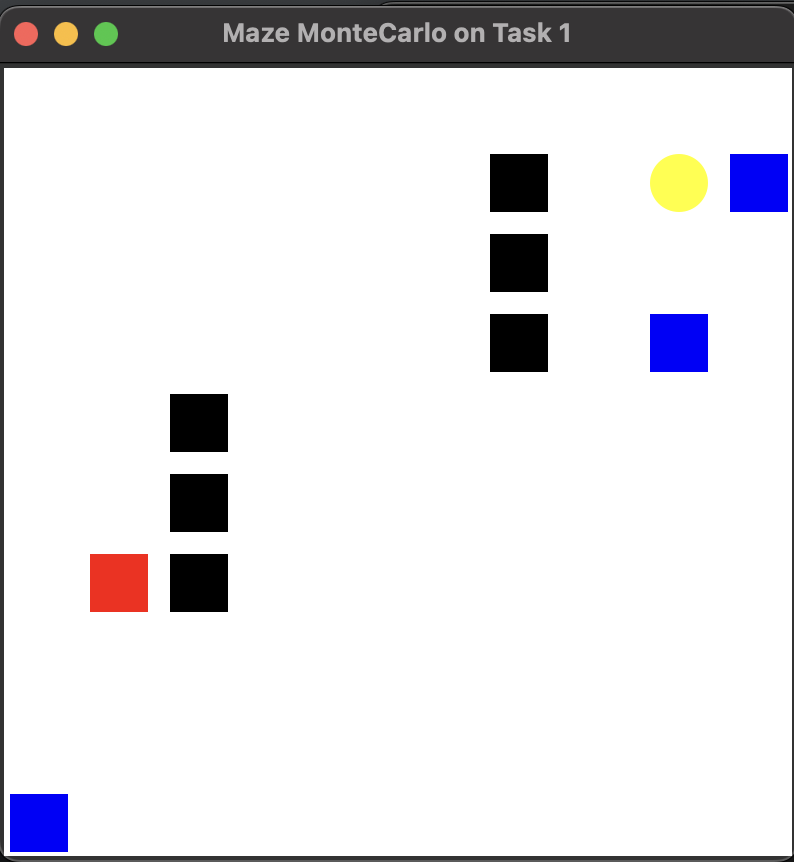
\includegraphics[width=\textwidth]{figs/task1.png}
        \caption{Task 1}
        \label{Fig_Task1}
    \end{subfigure}
    \hfill
    \begin{subfigure}{0.315\textwidth}
        \centering
        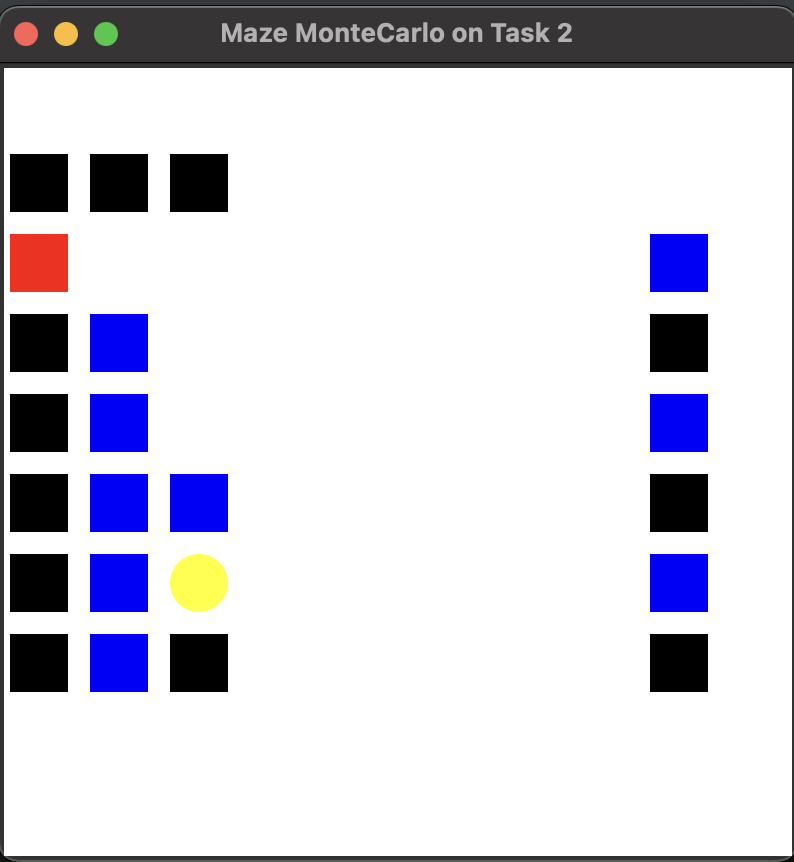
\includegraphics[width=\textwidth]{figs/task2.png}
        \caption{Task 2}
        \label{Fig_Task2}
    \end{subfigure}
    \hfill
    \begin{subfigure}{0.315\textwidth}
        \centering
        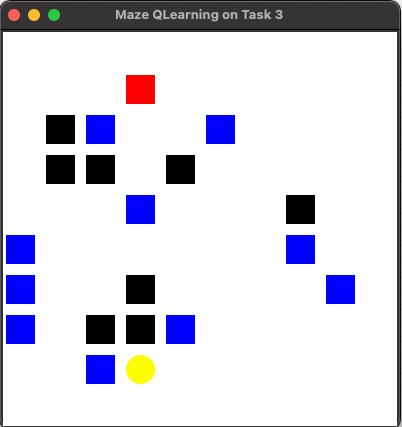
\includegraphics[width=\textwidth]{figs/task3.png}
        \caption{Task 3}
        \label{Fig_Task3}
    \end{subfigure}
    \label{Fig_Tasks}
\end{figure}
\end{frame}

\begin{frame}{Analytical Experiments: Results on Task 1}
  \centering
  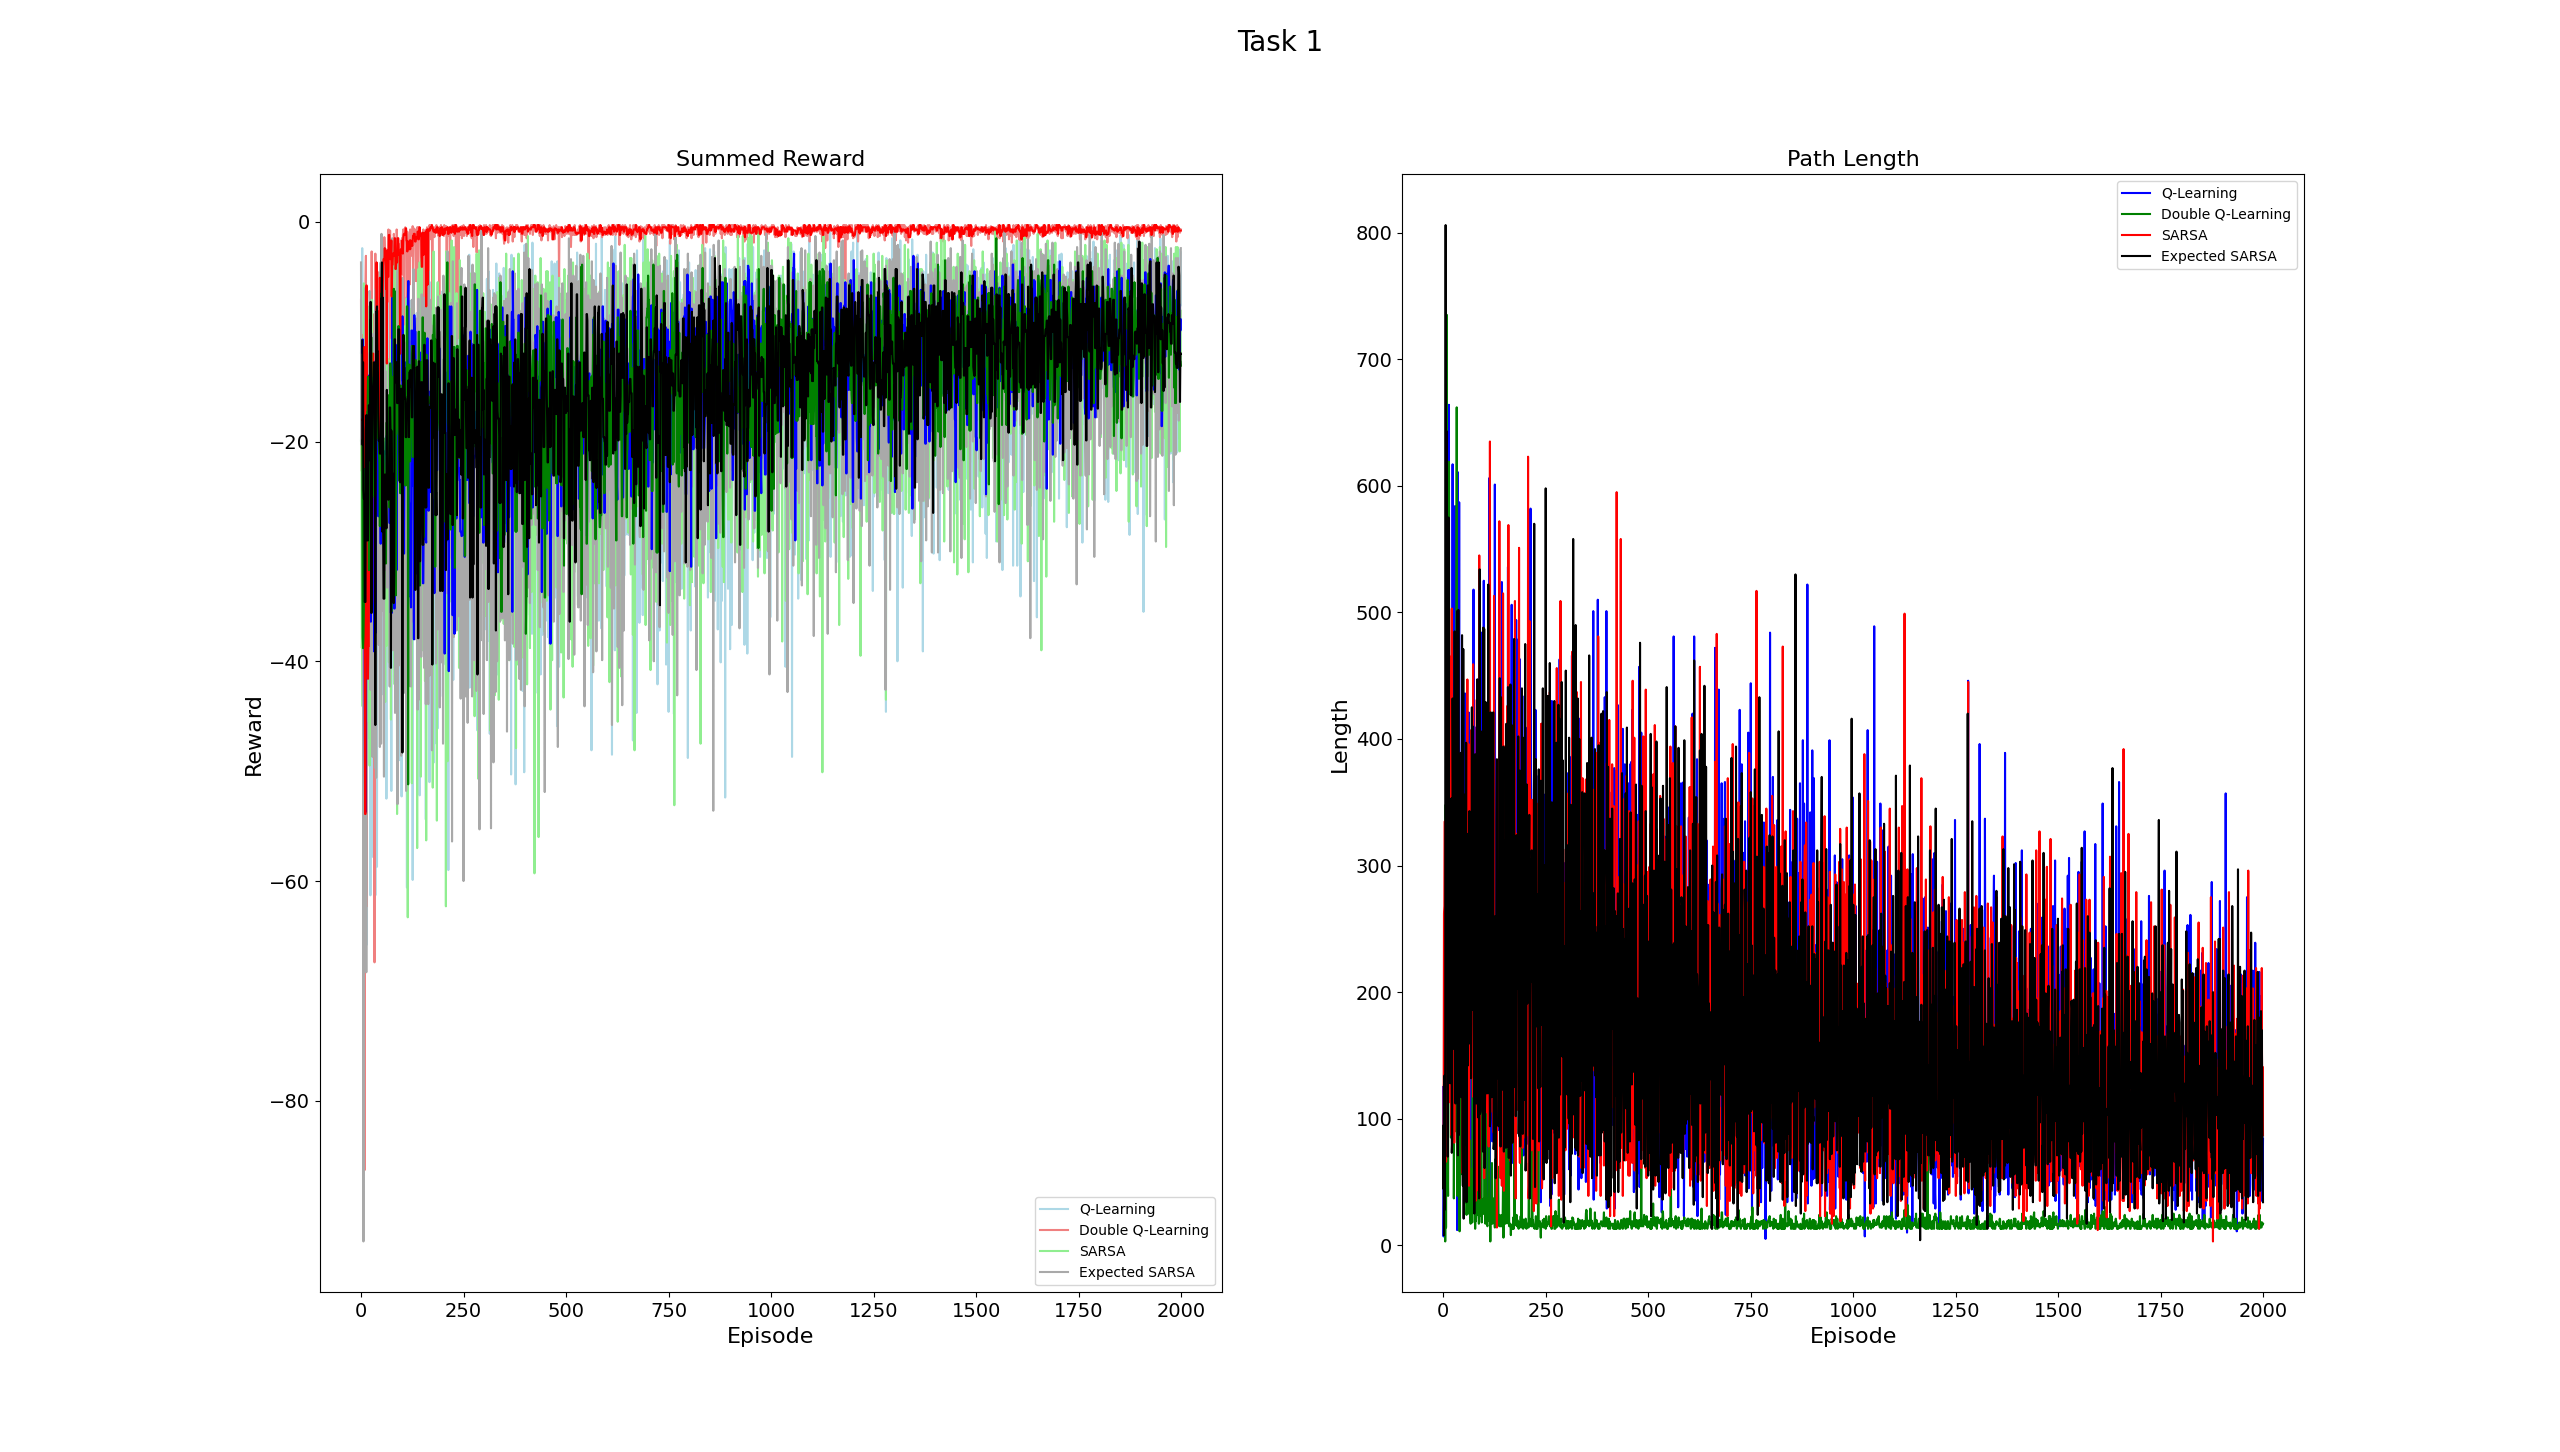
\includegraphics[width=0.99\textwidth]{figs/Task_1.png}
\end{frame}

\begin{frame}{Analytical Experiments: Results on Task 2}
  \centering
  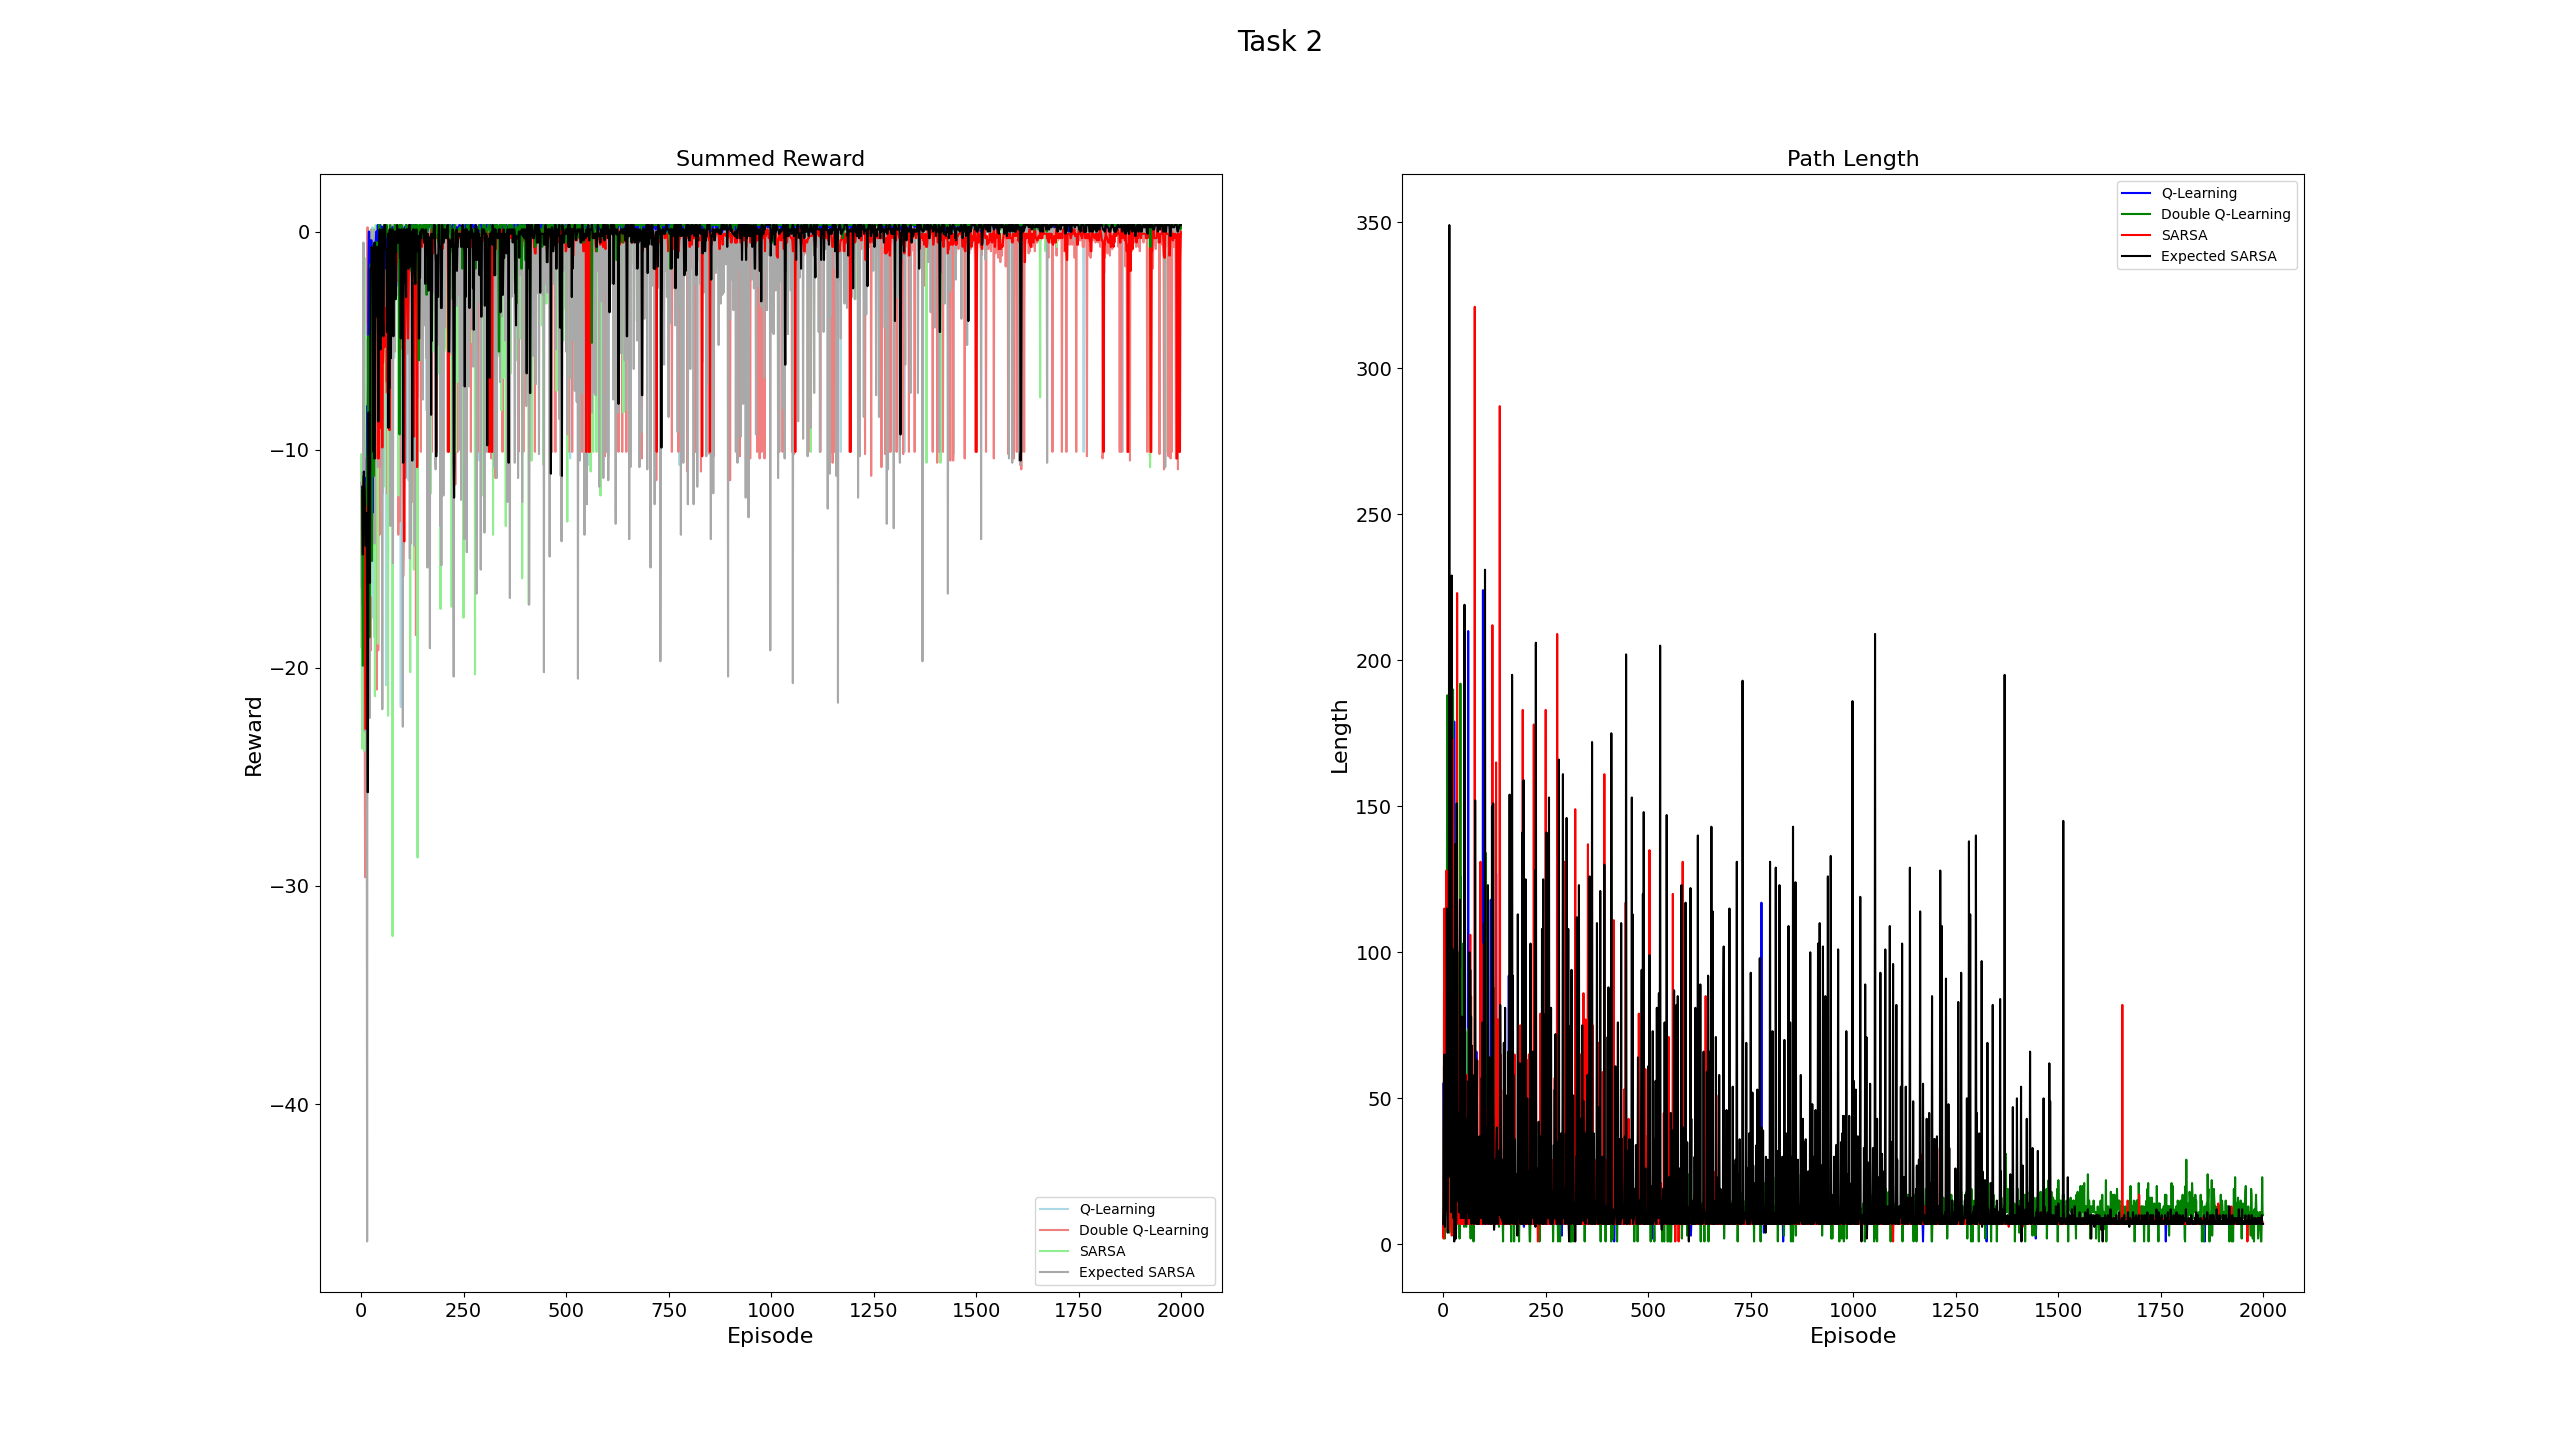
\includegraphics[width=0.99\textwidth]{figs/Task_2.png}
\end{frame}

\begin{frame}{Analytical Experiments: Results on Task 3}
  \centering
  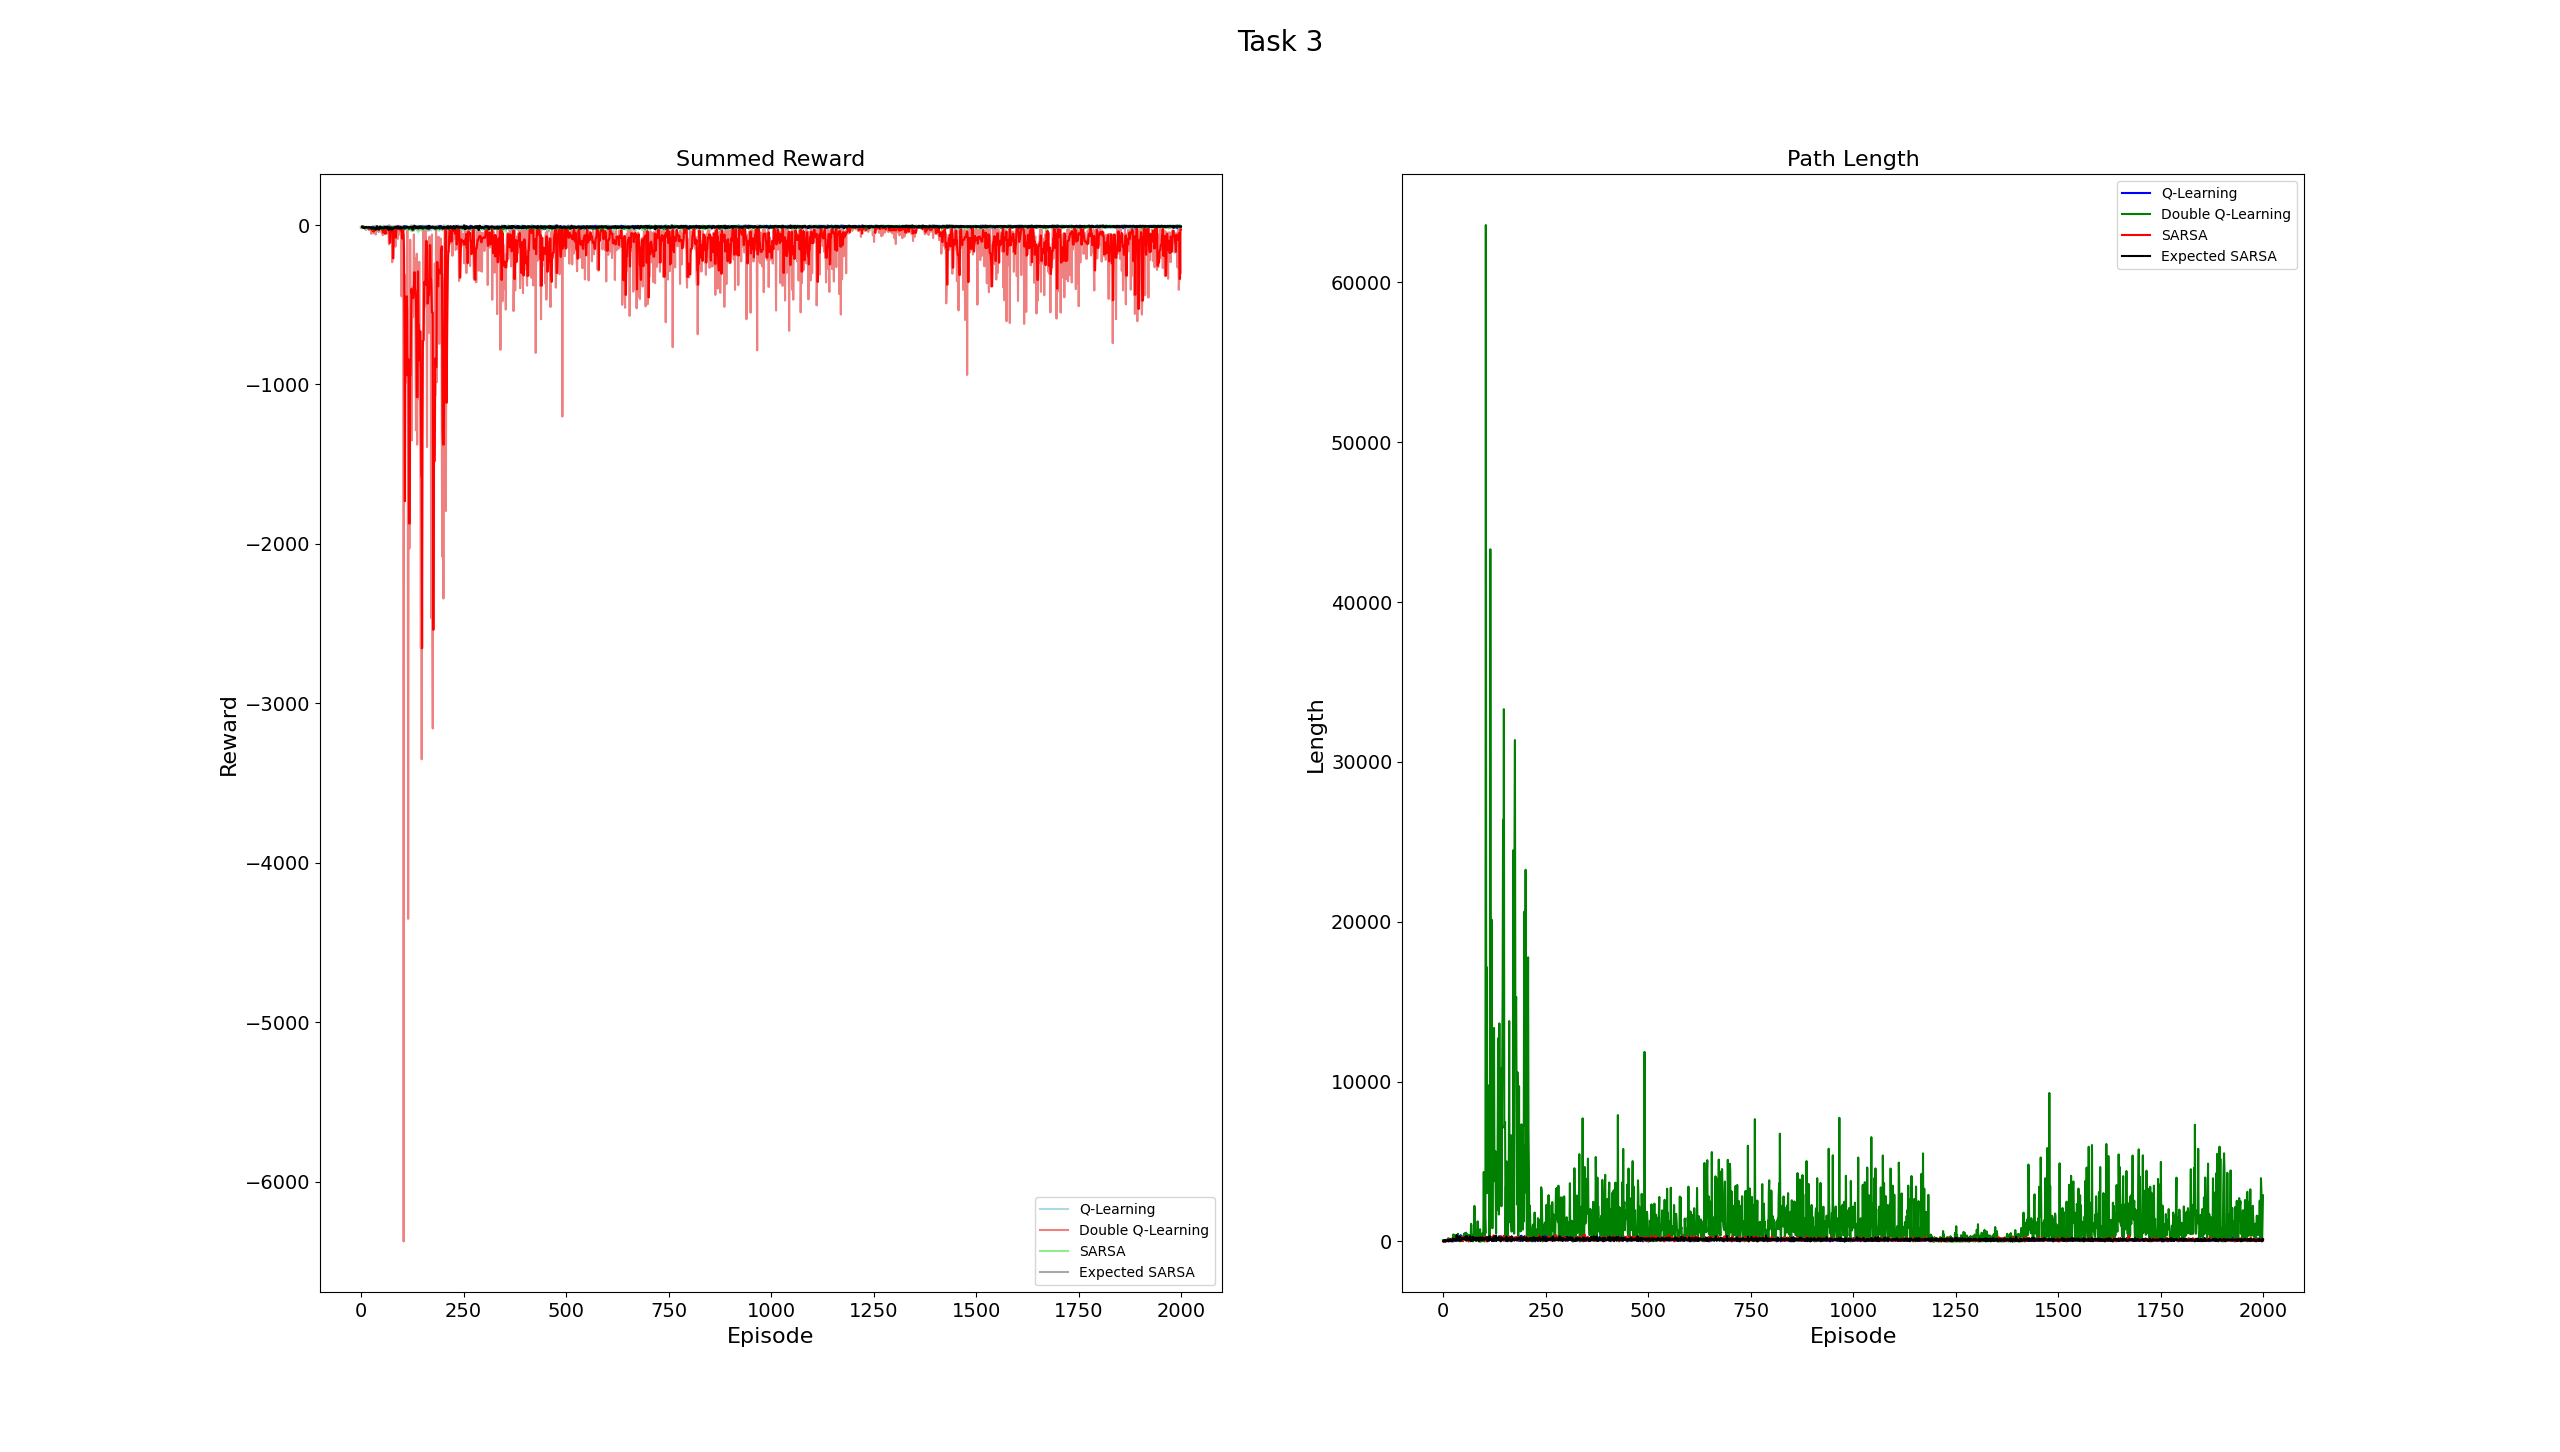
\includegraphics[width=0.99\textwidth]{figs/Task_3.png}
\end{frame}

\section{Analytical Experiments for DRL algorithms}
\begin{frame}{Analytical Experiments Overview}
  \begin{itemize}[<+->]
    \item \textbf{Purpose:} Evaluate the effects of different algorithmic choices on convergence and stability.
    \item \textbf{Experimental Setup:}
      \begin{itemize}[<+->]
        \item Controlled environments designed as a minimalist environment for decision-making in autonomous driving.
        \item Comparison of various algorithms: DQN, PPO, and A2C over three different environments -- \textbf{highway}, \textbf{intersection}, and the \textbf{racetrack} environments.
      \end{itemize}
    \item \textbf{Environments \& Tasks:}
      \begin{itemize}
        \item<+-> \emph{Highway fast:} In this task, the ego-vehicle is driving on a multilane highway populated with other vehicles. The agent's objective is to reach a high speed while avoiding collisions with neighbouring vehicles. Driving on the right side of the road is also rewarded.
        \item<+-> \emph{Intersection:} An intersection negotiation task with dense traffic.
        \item<+-> \emph{Racetrack:} A \textbf{continuous} control task involving lane-keeping and obstacle avoidance.
      \end{itemize}
  \end{itemize}
\end{frame}

\begin{frame}{Snapshots of Environments}
  \centering
  
\begin{figure}[t]
    \centering
    \begin{subfigure}{0.315\textwidth}
        \centering
        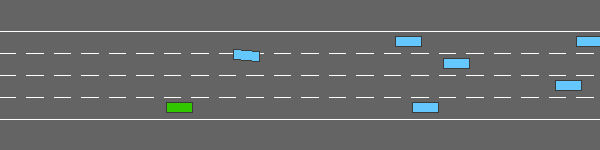
\includegraphics[width=\textwidth]{figs/highway.png}
        \caption{Highway task}
        \label{Fig_highway}
    \end{subfigure}
    \hfill
    \begin{subfigure}{0.315\textwidth}
        \centering
        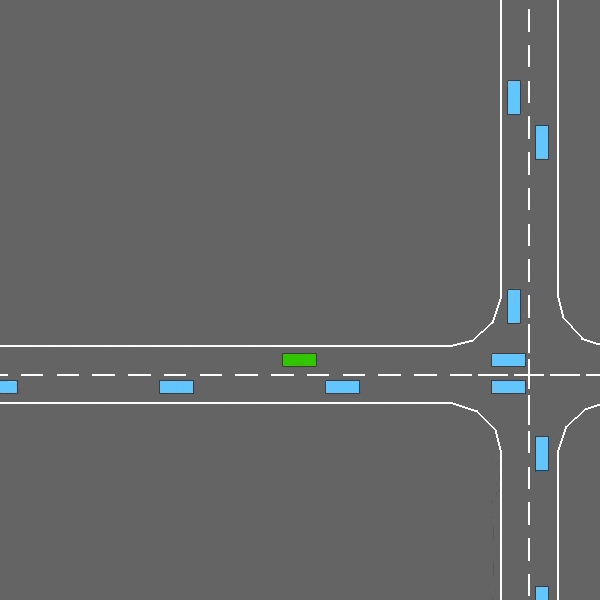
\includegraphics[width=\textwidth]{figs/intersection.png}
        \caption{Intersection task}
        \label{Fig_intersect}
    \end{subfigure}
    \hfill
    \begin{subfigure}{0.315\textwidth}
        \centering
        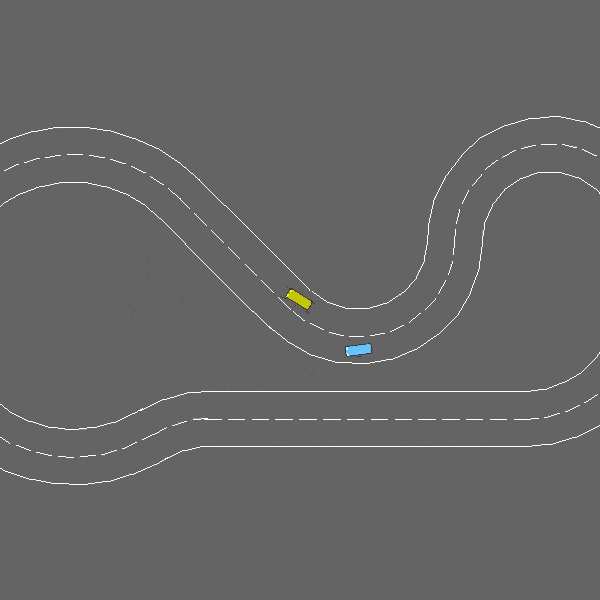
\includegraphics[width=\textwidth]{figs/racetrack.png}
        \caption{Racetrack task}
        \label{Fig_racetrack}
    \end{subfigure}
    \label{Fig_Highway_Farama}
\end{figure}
\end{frame}

\begin{frame}{Results \& Final Analysis -- Part I}
  \begin{itemize}[<+->]
  \item \textbf{Comparative Analysis Overview:}
    \begin{itemize}[<+->]
      \item Analysis was conducted across three tasks: \textbf{Highway-fast-v0}, \textbf{Intersection-v0}, and \textbf{Racetrack-v0}.
      \item Algorithms compared include DQN, PPO, and A2C.
    \end{itemize}
  \item \textbf{Highway-fast-v0:}
    \begin{itemize}[<+->]
      \item All algorithms performed well overall.
      \item \textbf{DQN:}
        \begin{itemize}[<+->]
          \item Exhibited more frequent lane changes compared to PPO and A2C.
          \item Had a higher crash rate of approximately 20\%.
        \end{itemize}
      \item \textbf{PPO and A2C:}
        \begin{itemize}[<+->]
          \item Achieved crash rates below 10\%.
          \item PPO consistently outperformed A2C.
        \end{itemize}
    \end{itemize}
    \end{itemize}
\end{frame}

\begin{frame}{Results \& Final Analysis -- Part II}
    \begin{itemize}
         \item \textbf{Intersection-v0:}
    \begin{itemize}[<+->]
      \item \textbf{PPO:} Significantly outperformed A2C with a crash rate of less than 10\%.
      \item \textbf{DQN and A2C:}
        \begin{itemize}[<+->]
          \item DQN experienced crash rates between 20--30\%.
          \item A2C had slightly less crash rate than DQN.
        \end{itemize}
    \end{itemize}
  \item \textbf{Racetrack-v0:}
    \begin{itemize}[<+->]
      \item Features a continuous action space.
      \item \textbf{PPO:} Delivered the best performance by efficiently overtaking non-ego vehicles.
      \item \textbf{A2C:} Demonstrated slower speeds and occasional failures to overtake.
      \item \textbf{DQN:}
        \begin{itemize}[<+->]
          \item Encountered significant challenges due to its design for discrete action spaces.
          \item Attempts to adapt using \texttt{DiscreteMetaActions} and \texttt{DiscreteActions} were unsuccessful.
          \item Resulted in erratic behavior (e.g., moving backward or circling) and frequent crashes.
        \end{itemize}
    \end{itemize}
\end{itemize}
\end{frame}

\section{Case Study 1: EV Routing \& Charging}
\begin{frame}{Case Study 1: EV Routing and Charging}
  \begin{itemize}[<+->]
    \item \textbf{Problem Overview:}
      \begin{itemize}[<+->]
        \item Efficient routing for electric vehicles under battery constraints and limited charging stations.
        \item Dynamic traffic conditions add to the complexity.
      \end{itemize}
  \end{itemize}
\end{frame}

\begin{frame}{System Figure}
  \centering
  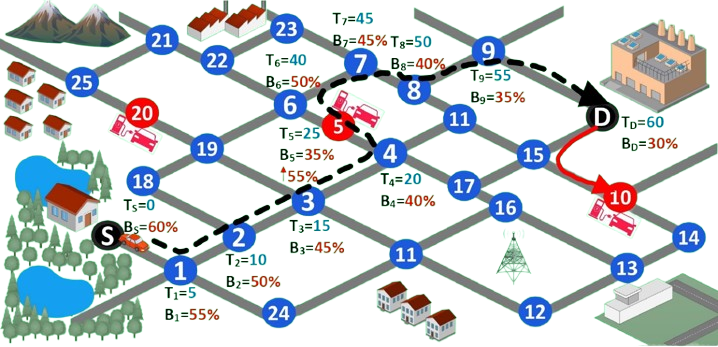
\includegraphics[width=0.99\textwidth]{figs/System_Model2_page-0001-removebg-preview (1).png}
\end{frame}

\begin{frame}{MDP Components}
  \begin{itemize}
    \item \textbf{Agent:} The EV itself acts as the decision-maker, navigating a dynamic urban environment to minimize travel time.
    \pause
    \item \textbf{States:}
      \begin{itemize}
        \item Location: Current node in the road network
        \item Battery Level: Current charge of the EV
        \item \textit{Terminal State:} Reaching the destination ends the journey.
      \end{itemize}
    \pause
    \item \textbf{Actions (Discrete):}
      \begin{itemize}
        \item Movement: Transition from one node to an adjacent node.
        \item Recharging: Option to recharge at available charging stations.
      \end{itemize}
    \pause
    \item \textbf{Reward:}
      \begin{itemize}
        \item Time Cost: Negative reward equal to travel and charging durations (80\% - current battery level).
        \item Penalty: Additional penalty if battery level drops below 20\%.
      \end{itemize}
  \end{itemize}
\end{frame}

\begin{frame}{Case Study 1: Approaches and Key Findings}
  \begin{itemize}[<+->]
    \item \textbf{Algorithms:}
      \begin{itemize}[<+->]
        \item \emph{Q-Learning (QL)}
        \item \emph{TERC-augmented Q-Learning (TQL)}
        \item \emph{Deep Q-Learning (DQL)}
      \end{itemize}
    \item \textbf{Key Findings:}
      \begin{itemize}[<+->]
        \item TQL reduces travel distance and charging overhead.
        \item DQL scales better for larger networks and dynamic scenarios.
        \item All approaches converged to the same output.
      \end{itemize}
  \end{itemize}
\end{frame}

\section{Case Study 2: Vehicle Patrol Scheduling}
\begin{frame}{Case Study 2: Vehicle Patrol Scheduling}
  \begin{itemize}[<+->]
    \item \textbf{Problem Overview:}
      \begin{itemize}[<+->]
        \item Scheduling patrol vehicles to cover locations.
        \item Constraints include rest time in the depot, re-visit intervals, operation limit, etc.
        \item Vehicles must leave from the depot, visit as many locations as can wrt the constraints, and come back to the depot.
      \end{itemize}
  \end{itemize}
\end{frame}

\begin{frame}{System Figure}
  \centering
  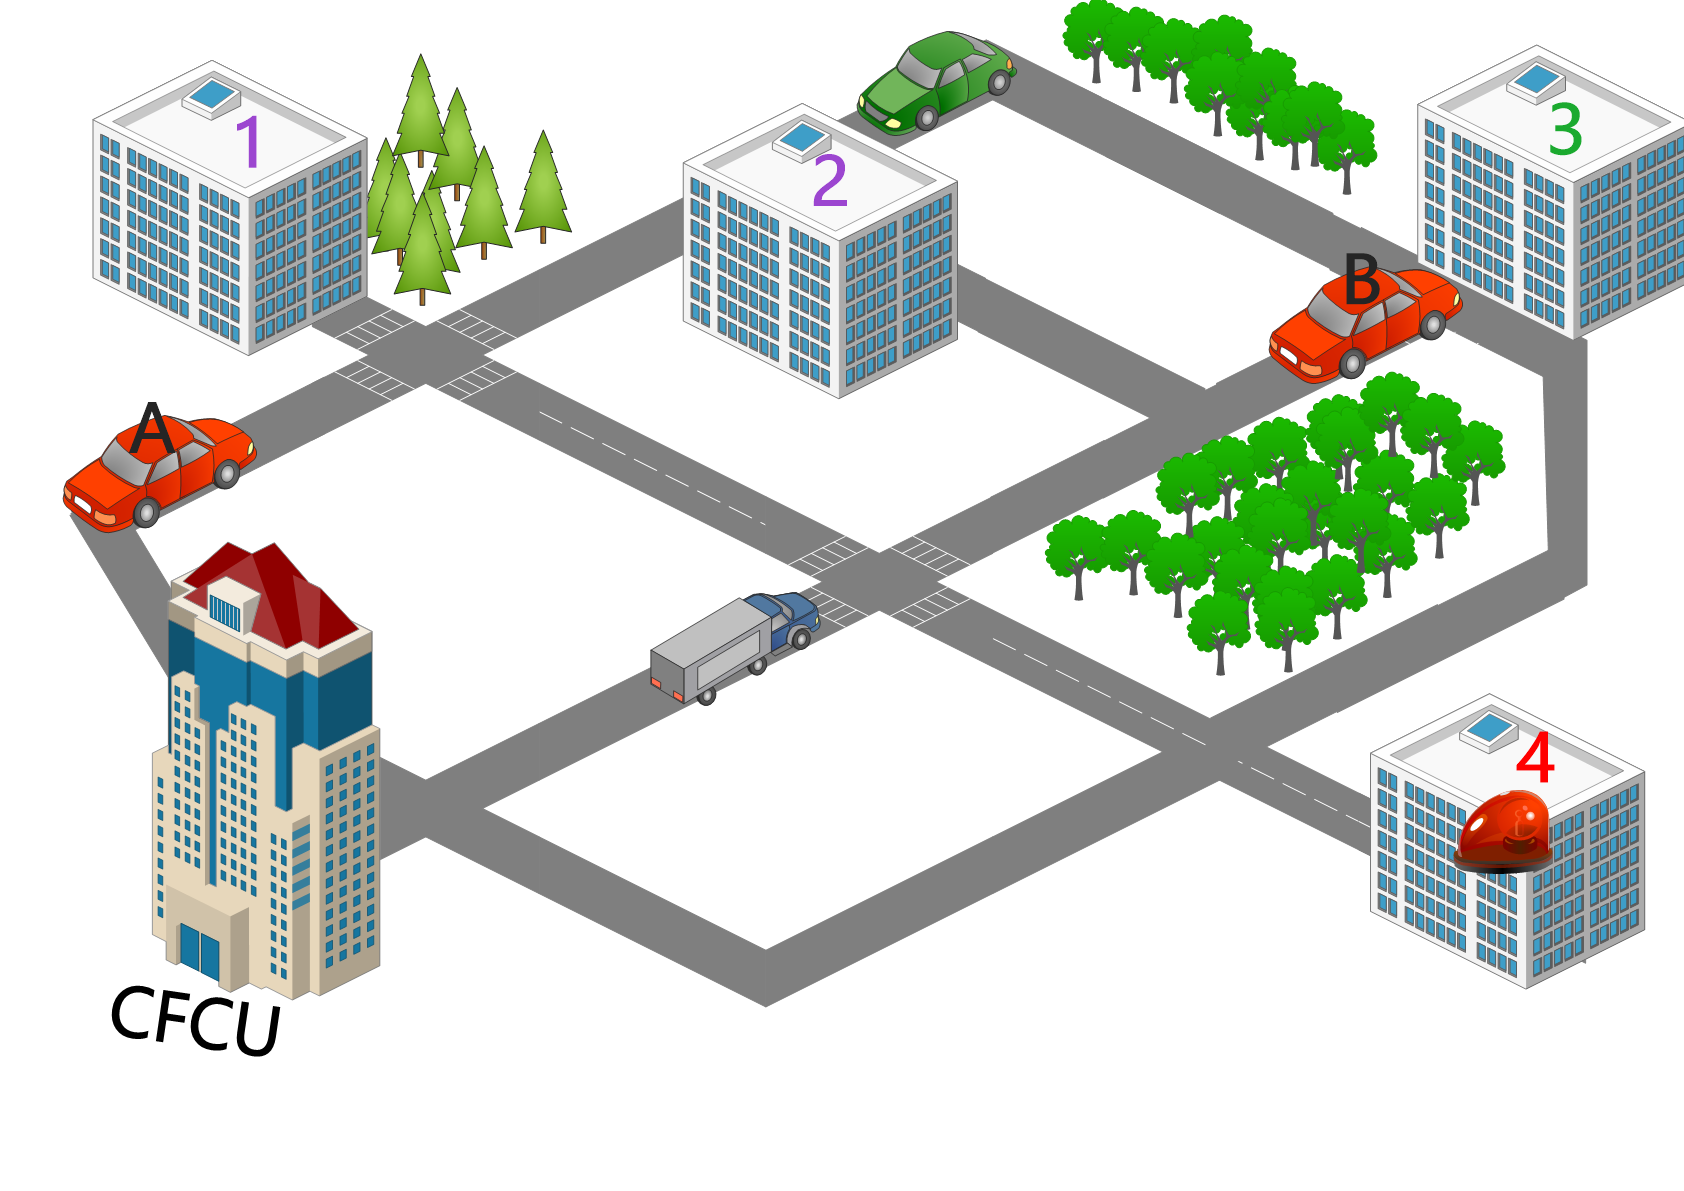
\includegraphics[width=0.9\textwidth]{figs/P4O (1).png}
\end{frame}

\begin{frame}{Basic Constraints}
  \begin{itemize}
    \item \textbf{Initial Location Constraint:} Vehicles must start their journey at the depot.
    \pause
    \item \textbf{Operation Shift Constraint:} Visits are scheduled within designated shifts.
    \pause
    \item \textbf{Single Vehicle Constraint:} A vehicle can only be at one location at a time.
    \pause
    \item \textbf{Single Location Constraint:} No location is patrolled by more than one vehicle simultaneously.
    \pause
    \item \textbf{Path Feasibility Constraint:} Vehicles can only travel along valid, connected routes.
    \pause
    \item \textbf{Depot Visit Constraint:} Vehicles must return to the depot at least once during each shift.
  \end{itemize}
\end{frame}

\begin{frame}{Time and Scheduling Constraints}
  \begin{itemize}
    \item \textbf{Depot Rest Time Constraint:} Vehicles are required to take a minimum rest period at the depot.
    \pause
    \item \textbf{Vehicle Visit Time Constraint:} Start times for each visit depend on previous visits and travel durations.
    \pause
    \item \textbf{Rest Time End Constraint:} Vehicles cannot resume patrol until the required rest period is complete.
    \pause
    \item \textbf{Rest Time Start Constraint:} Rest begins immediately upon arrival at the depot.
  \end{itemize}
\end{frame}

\begin{frame}{Coverage and Continuity Constraints}
  \begin{itemize}
    \item \textbf{Maximum Shifts Constraint:} Limits the number of visits or patrols per shift.
    \pause
    \item \textbf{Vehicle Arrival Constraint:} A vehicle must arrive at a location before starting its patrol there.
    \pause
    \item \textbf{Consecutive Visits Gap Constraint:} Enforces a maximum allowable time gap between successive visits to a location.
    \pause
    \item \textbf{Minimum Patrolling Duration Constraint:} Each visit must include a minimum time to ensure sufficient coverage.
    \pause
    \item \textbf{Shifts Order Constraint:} Patrol shifts must occur sequentially with the required time gaps between them.
  \end{itemize}
\end{frame}

\begin{frame}{Case Study 2: Approaches and Key Findings}
  \begin{itemize}[<+->]
    \item \textbf{Approaches Evaluated:}
      \begin{itemize}[<+->]
        \item \emph{Classical Optimization}
        \item \emph{Heuristic Methods:} Adaptive Hill-Climbing and Genetic Algorithms, since VPS is an NP-hard problem (TSP).
      \end{itemize}
    \item \textbf{Results:}
      \begin{itemize}[<+->]
        \item The optimization model works perfectly for small instances.
        \item AHBPS efficiently covers a decent portion of the locations with fast response and scheduling times.
        \item GDVPS performs well in terms of both coverage and response time.
      \end{itemize}
  \end{itemize}
\end{frame}

\begin{frame}{Case Study 2: Approaches and Key Findings (Figures)}
    \begin{figure}[t]
    \centering
    \begin{subfigure}{0.315\textwidth}
        \centering
        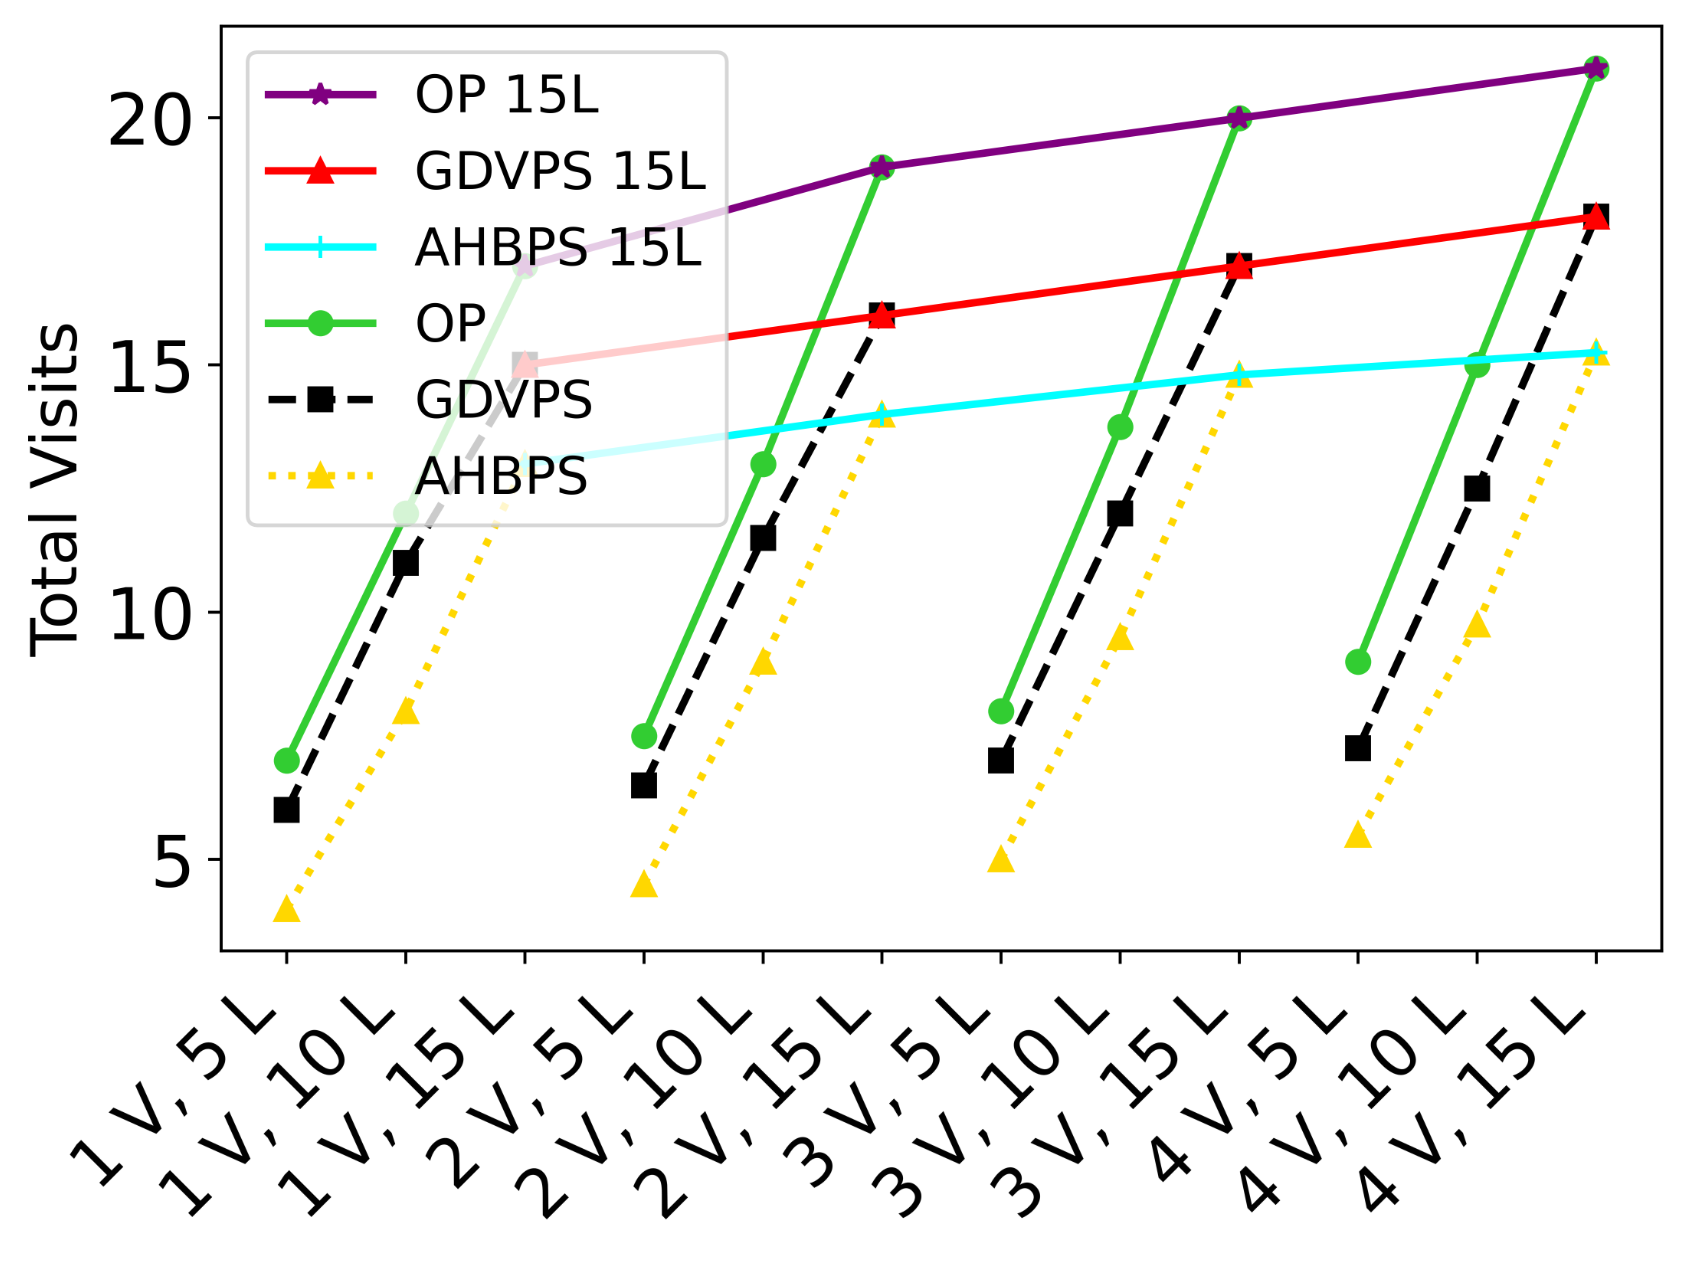
\includegraphics[width=\textwidth]{figs/all_acc.png}
        \caption{}
    \end{subfigure}
    \hfill
    \begin{subfigure}{0.315\textwidth}
        \centering
        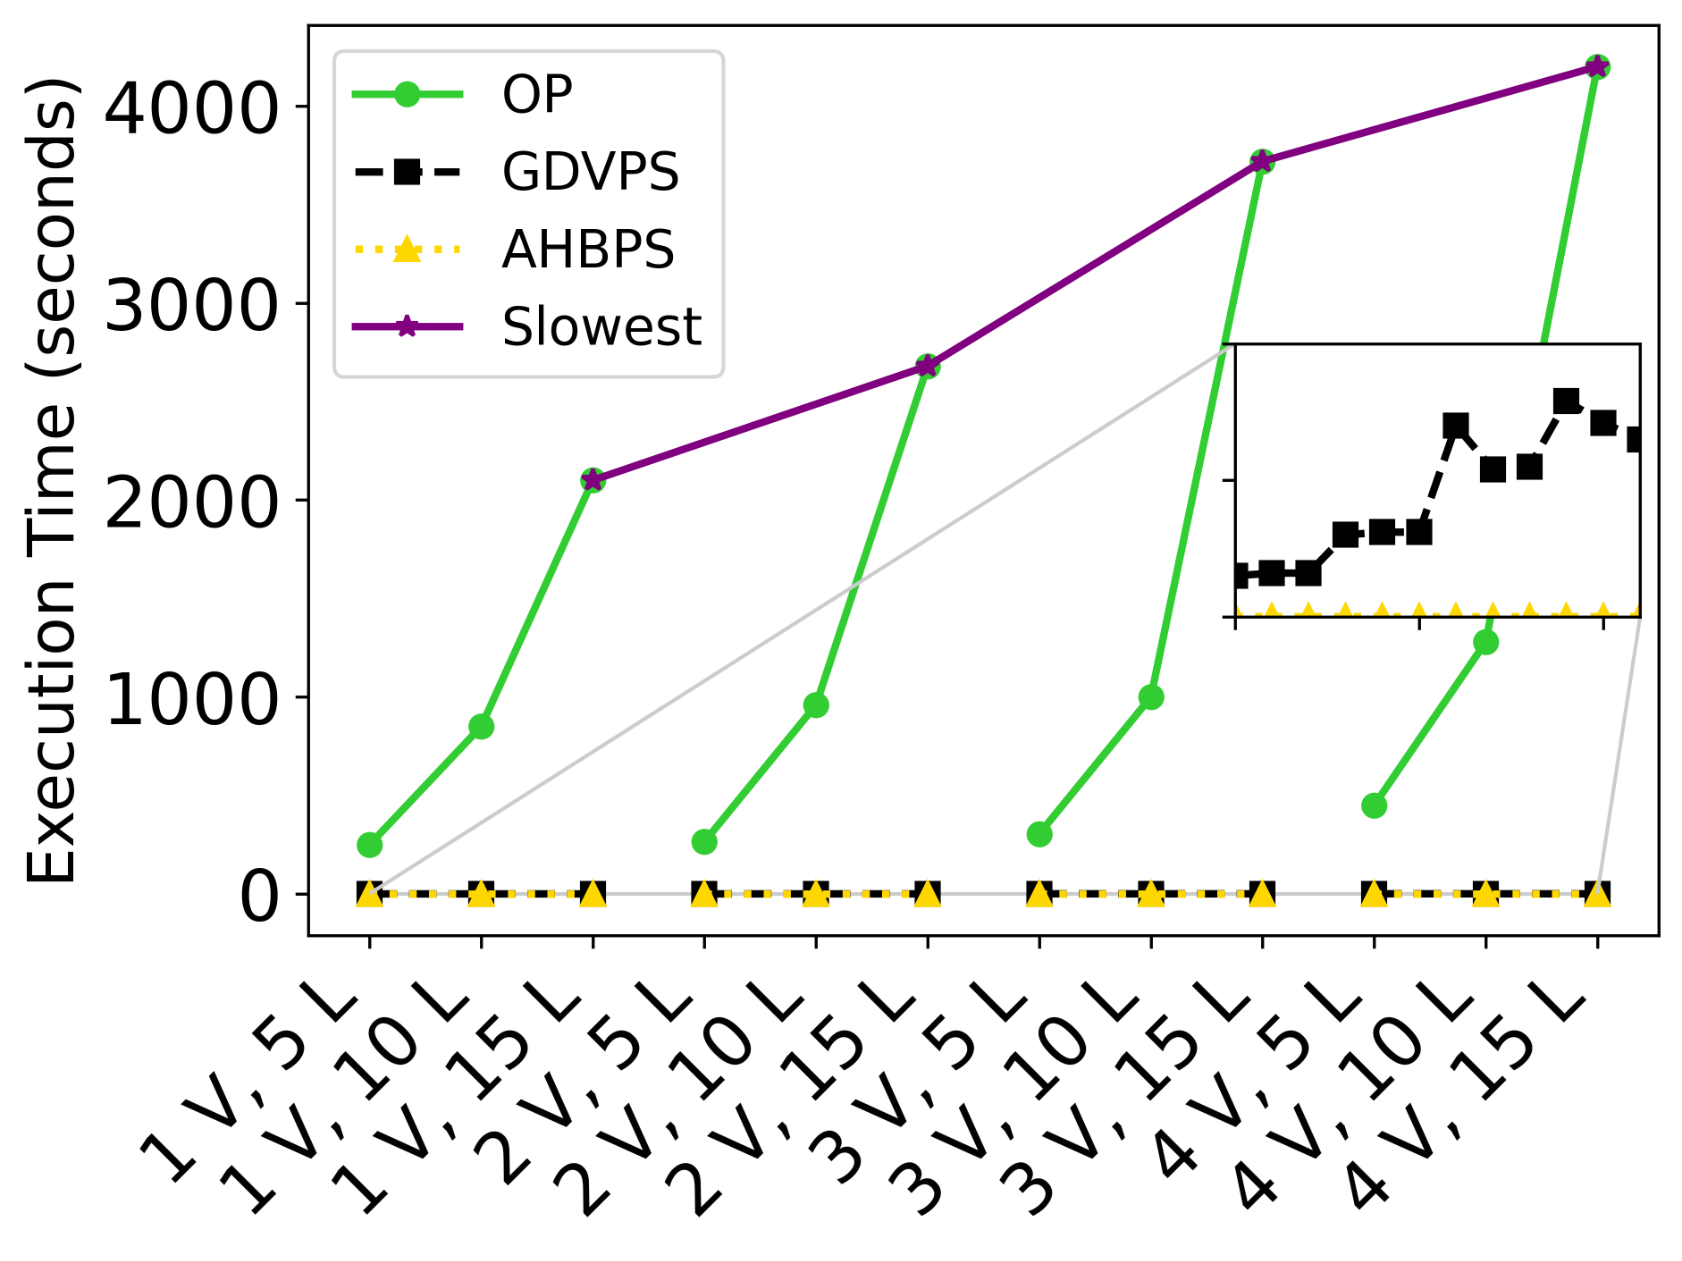
\includegraphics[width=\textwidth]{figs/all_exec.png}
        \caption{}
    \end{subfigure}
    \hfill
    \begin{subfigure}{0.315\textwidth}
        \centering
        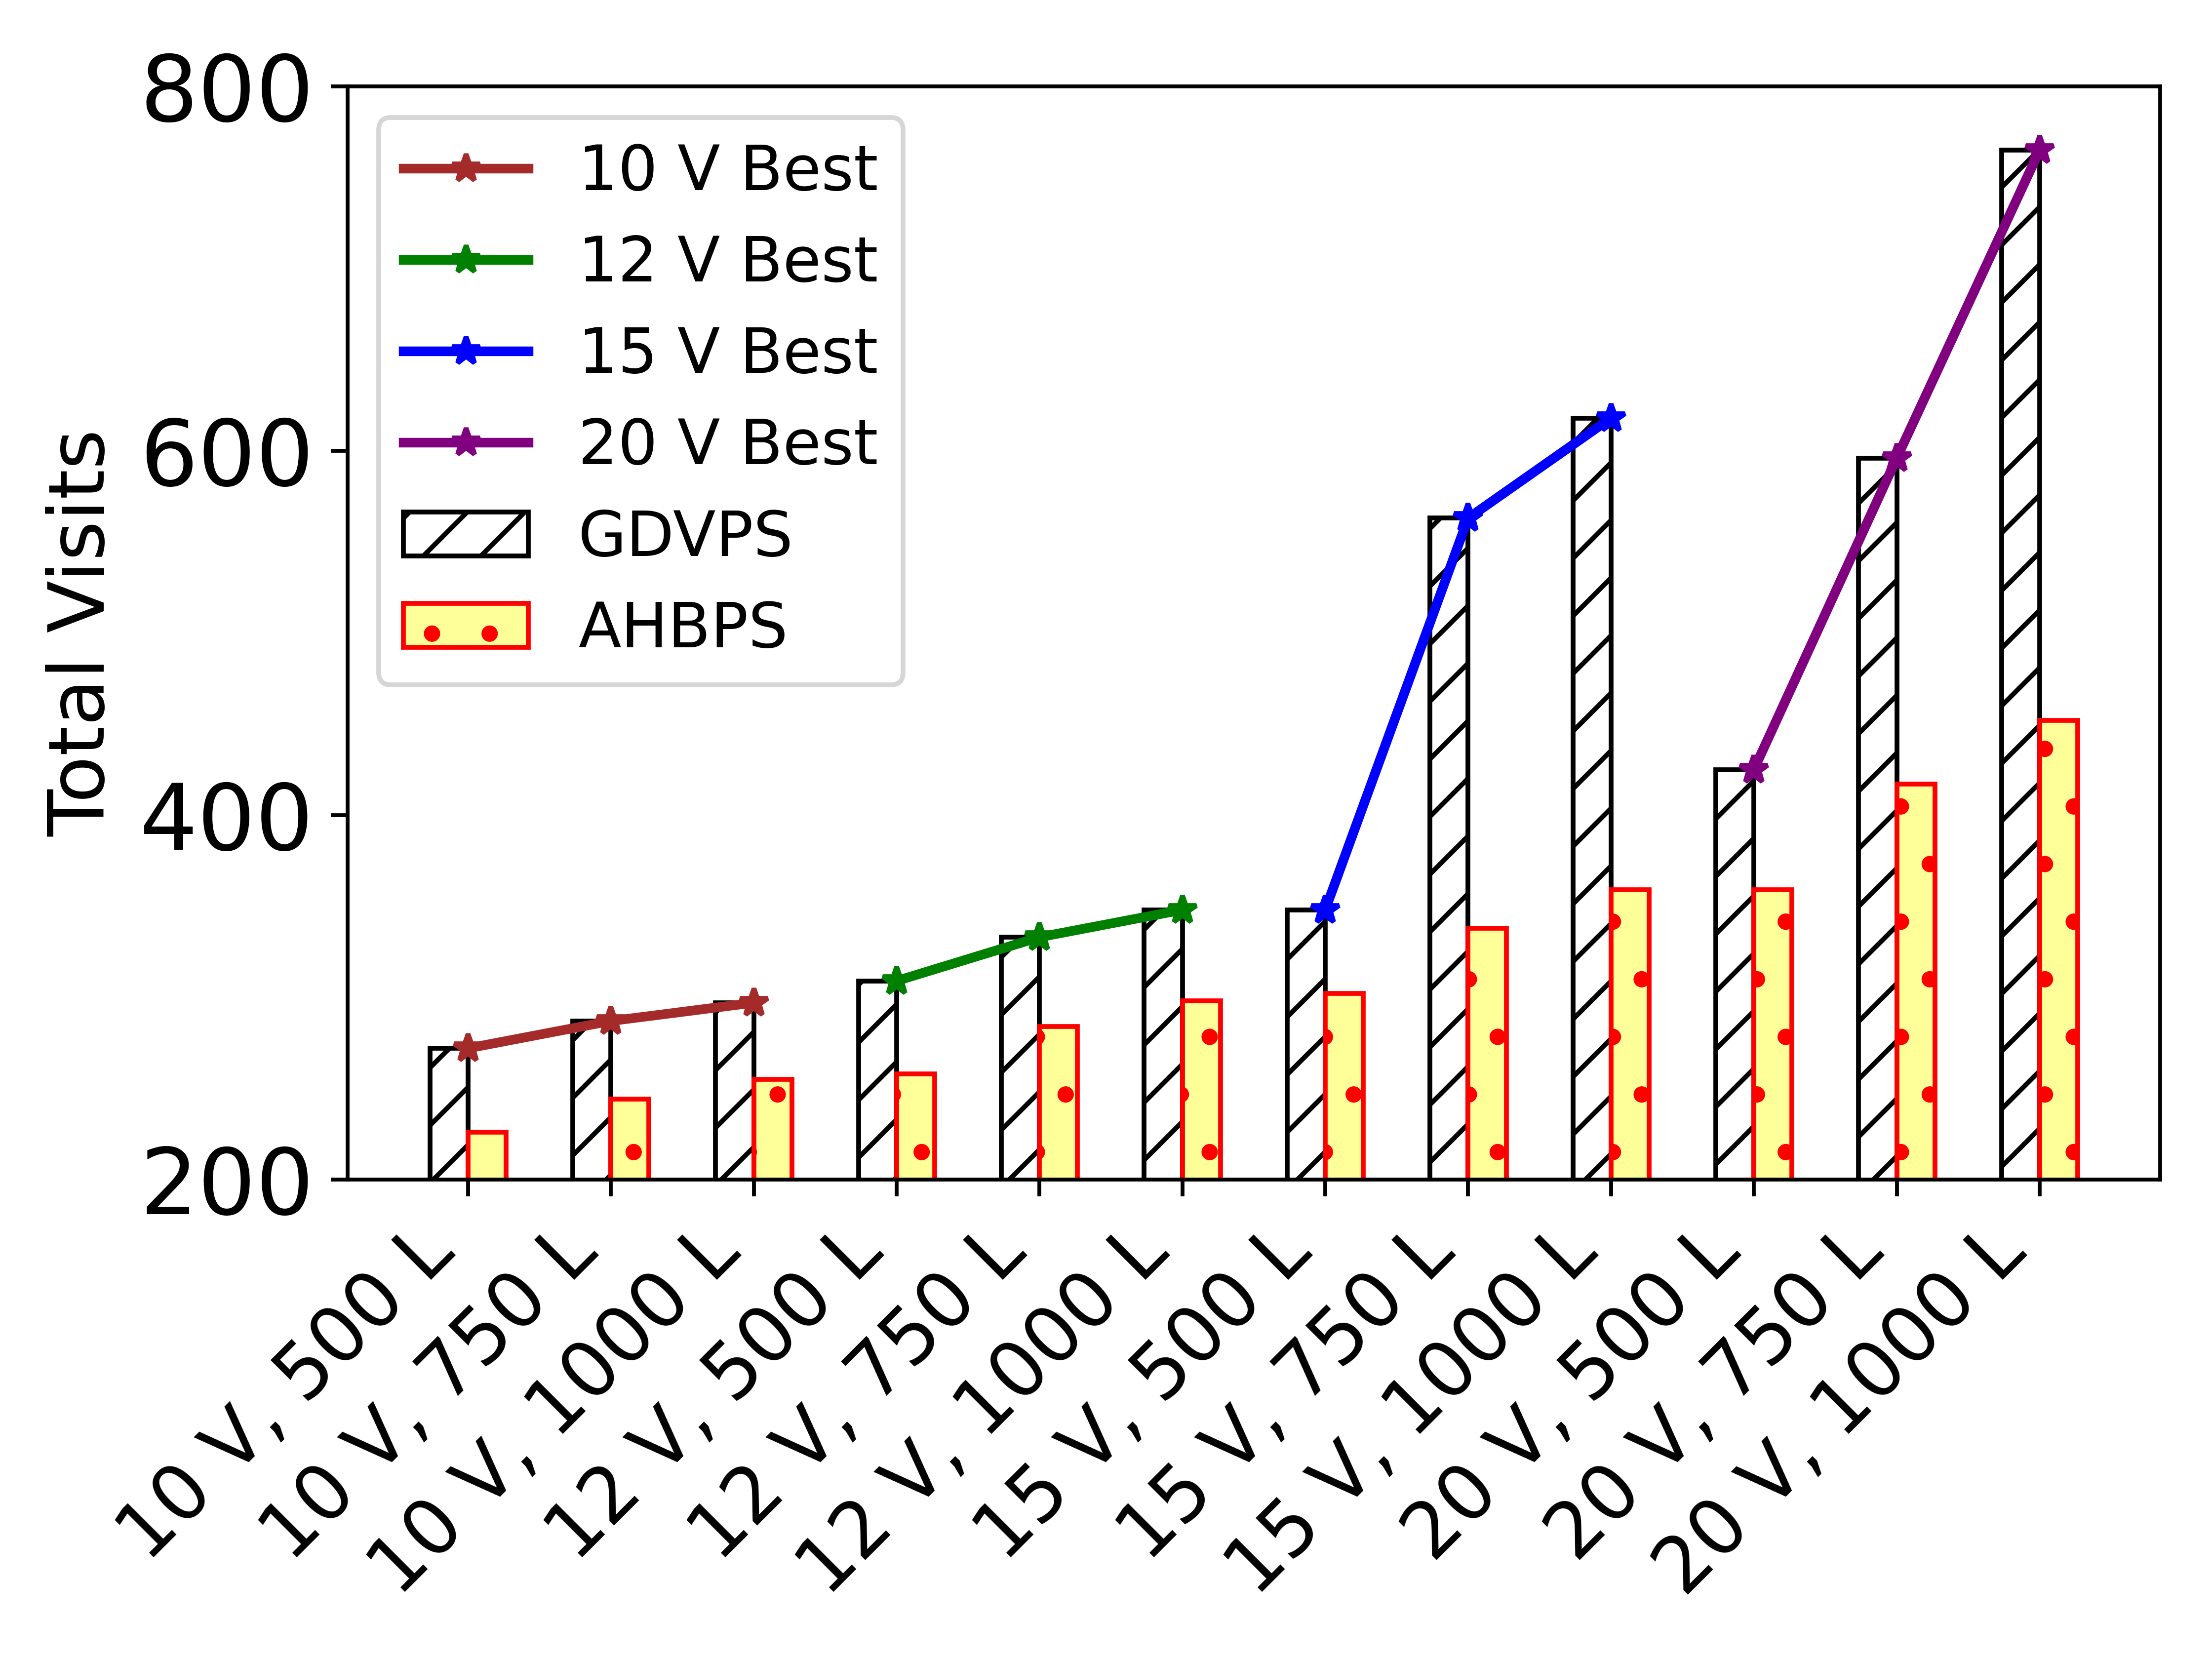
\includegraphics[width=\textwidth]{figs/large_acc_corrected (1).png}
        \caption{}
    \end{subfigure}
    \label{Fig_Highway_Farama}
\end{figure}
\end{frame}

\begin{frame}{$\mathcal{P}^4\mathcal{O}$'s MDP}
  \begin{itemize}[<+->]
    \item \textbf{Agent:} Central Fleet Control Unit (CFCU) at the depot, responsible for determining optimal vehicle routes, handling emergencies, and dynamically reorganizing schedules.
    \pause
    \item \textbf{State:} Comprises both discrete and continuous elements:
      \begin{itemize}[<+->]
        \item \emph{Discrete:} Set of visited locations, current shift number, and emergency status.
        \item \emph{Continuous:} Last visit time for each location, remaining shift time for each vehicle.
      \end{itemize}
    \pause
    \item \textbf{Actions:} Selecting the next accessible location for each vehicle from a predefined set.
    \pause
    \item \textbf{Reward:}
      \begin{itemize}[<+->]
        \item Small positive reward for each visited location (+0.5).
        \item Penalty (-10) if an emergency is not addressed within the allowable response time.
        \item Penalty for violating the revisit time.
      \end{itemize}
    \pause
  \end{itemize}
\end{frame}

\begin{frame}{Case Study 2: RL-Based Approach: $\mathcal{P}^4\mathcal{O}$}
  \begin{itemize}[<+->]
    \item \textbf{Approach Evaluated:}
      \begin{itemize}[<+->]
        \item \emph{RL-Based Approach:} Patrol Planning with PPO.
      \end{itemize}
    \item \textbf{Results:}
      \begin{itemize}[<+->]
        \item $\mathcal{P}^4\mathcal{O}$ adapts in real time to emergency calls and traffic changes.
        \item $\mathcal{P}^4\mathcal{O}$ covers more locations per shift and in total.
      \end{itemize}
  \end{itemize}
\end{frame}

\begin{frame}{Case Study 2: RL-based Approach Key Findings}
    \begin{figure}[t]
    \centering
    \begin{subfigure}{0.48\textwidth}
        \centering
        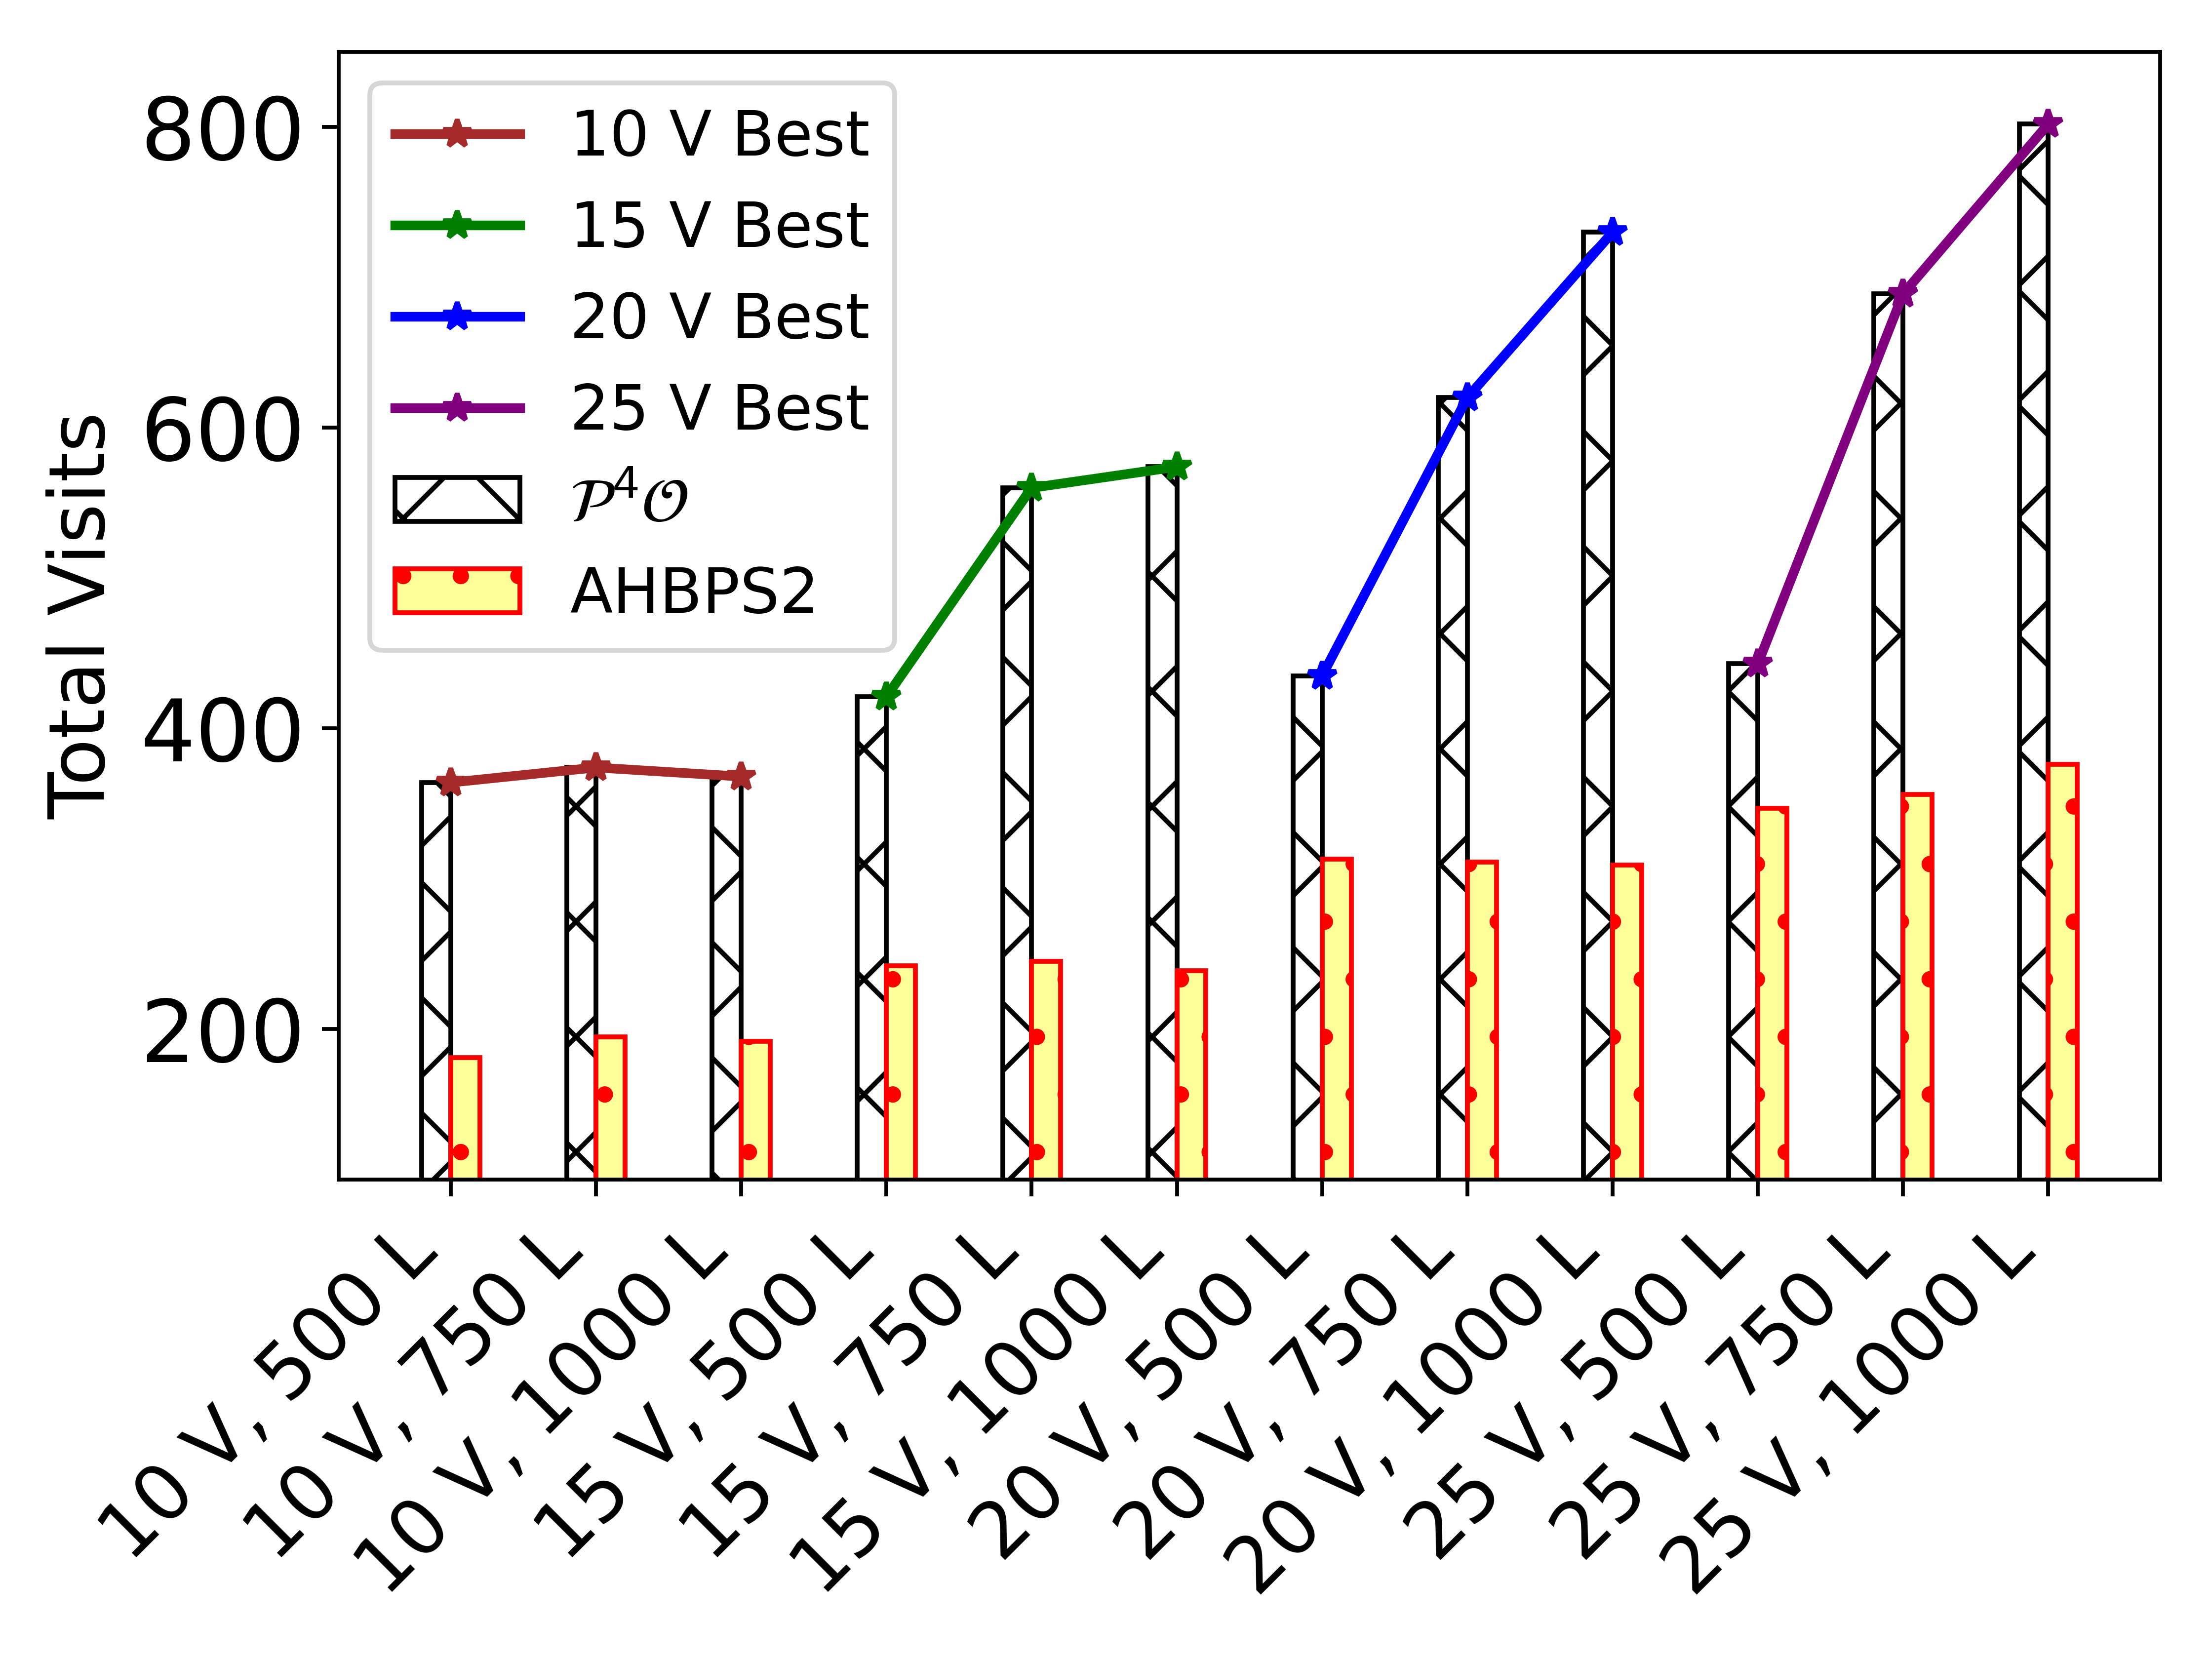
\includegraphics[width=\textwidth]{figs/large_acc_corrected (2).png}
        \caption{}
    \end{subfigure}
    \hfill
    \begin{subfigure}{0.48\textwidth}
        \centering
        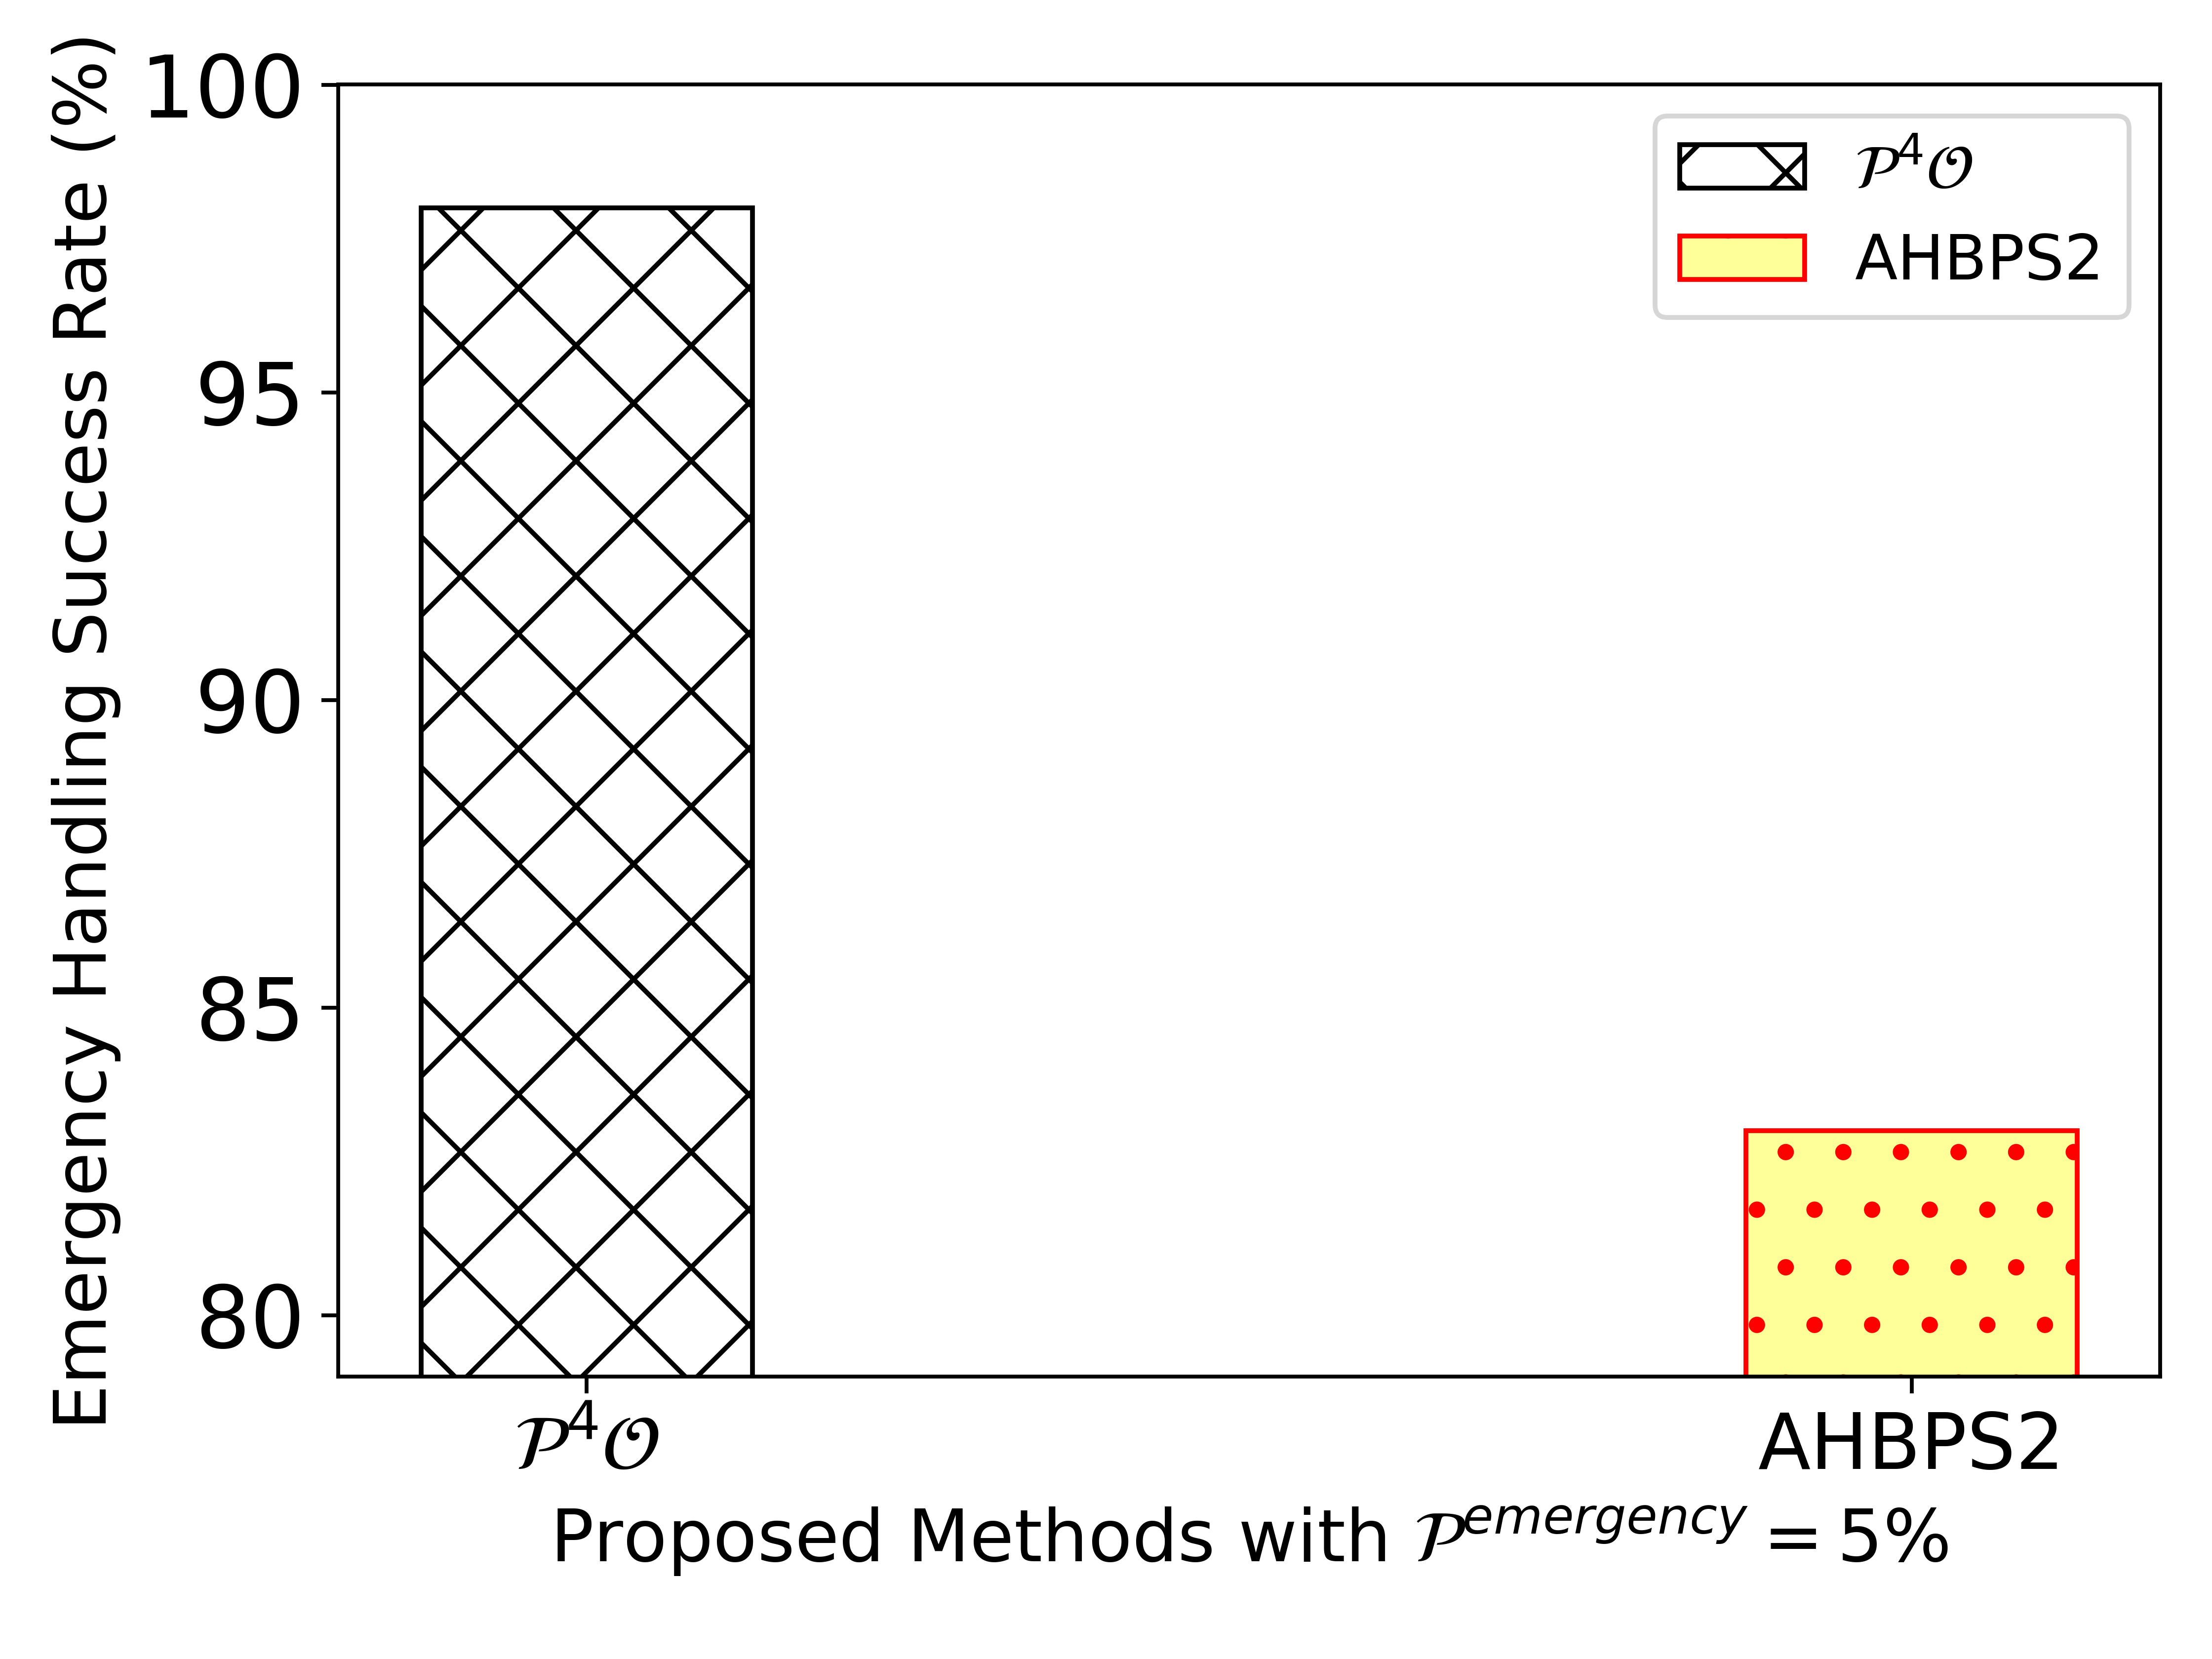
\includegraphics[width=\textwidth]{figs/emergency_handling.png}
        \caption{}
    \end{subfigure}
\end{figure}
\end{frame}

\section{Results and Discussion}
\begin{frame}{Overall Results and Discussion}
  \begin{itemize}[<+->]
    \item \textbf{Analytical Experiments:}
      \begin{itemize}[<+->]
        \item Sensitivity of convergence to exploration strategies and reward shaping.
        \item Actionable insights for parameter tuning in larger-scale applications.
      \end{itemize}
    \item \textbf{EV Routing \& Charging:}
      \begin{itemize}[<+->]
        \item TQL showed marked improvements over pure tabular methods.
        \item DQL demonstrated scalability and robust performance under dynamic conditions.
      \end{itemize}
    \item \textbf{Vehicle Patrol Scheduling:}
      \begin{itemize}[<+->]
        \item The $\mathcal{P}^4\mathcal{O}$ framework adapts well to real-time changes, outperforming classical and heuristic methods.
      \end{itemize}
    \item \textbf{Key Insight:} Hybrid approaches that integrate analytical insights with RL strategies provide a practical path for real-world deployments.
  \end{itemize}
\end{frame}

\section{Conclusion and Future Work}
\begin{frame}{Conclusion and Future Work}
  \begin{itemize}[<+->]
    \item \textbf{Contributions:}
      \begin{itemize}[<+->]
        \item Integration of analytical experiments with RL applications in EV routing and vehicle patrol scheduling.
        \item Demonstration of how analytical insights can guide the design of scalable, stable RL systems.
      \end{itemize}
    \item \textbf{Future Directions:}
      \begin{itemize}[<+->]
        \item Further investigation into hybrid RL models.
        \item Extension to more complex real-world scenarios with real-time data integration.
      \end{itemize}
  \end{itemize}
\end{frame}

\begin{frame}{Acknowledgment}
\centering
Thanks to all the co-authors!
\end{frame}

\begin{frame}{Questions \& Discussion}
  \centering
  \Large{Thank you! \\[1em] Questions?}
\end{frame}

\end{document}
